\documentclass[twoside]{book}

% Packages required by doxygen
\usepackage{fixltx2e}
\usepackage{calc}
\usepackage{doxygen}
\usepackage[export]{adjustbox} % also loads graphicx
\usepackage{graphicx}
\usepackage[utf8]{inputenc}
\usepackage{makeidx}
\usepackage{multicol}
\usepackage{multirow}
\PassOptionsToPackage{warn}{textcomp}
\usepackage{textcomp}
\usepackage[nointegrals]{wasysym}
\usepackage[table]{xcolor}

% Font selection
\usepackage[T1]{fontenc}
\usepackage[scaled=.90]{helvet}
\usepackage{courier}
\usepackage{amssymb}
\usepackage{sectsty}
\renewcommand{\familydefault}{\sfdefault}
\allsectionsfont{%
  \fontseries{bc}\selectfont%
  \color{darkgray}%
}
\renewcommand{\DoxyLabelFont}{%
  \fontseries{bc}\selectfont%
  \color{darkgray}%
}
\newcommand{\+}{\discretionary{\mbox{\scriptsize$\hookleftarrow$}}{}{}}

% Page & text layout
\usepackage{geometry}
\geometry{%
  a4paper,%
  top=2.5cm,%
  bottom=2.5cm,%
  left=2.5cm,%
  right=2.5cm%
}
\tolerance=750
\hfuzz=15pt
\hbadness=750
\setlength{\emergencystretch}{15pt}
\setlength{\parindent}{0cm}
\setlength{\parskip}{3ex plus 2ex minus 2ex}
\makeatletter
\renewcommand{\paragraph}{%
  \@startsection{paragraph}{4}{0ex}{-1.0ex}{1.0ex}{%
    \normalfont\normalsize\bfseries\SS@parafont%
  }%
}
\renewcommand{\subparagraph}{%
  \@startsection{subparagraph}{5}{0ex}{-1.0ex}{1.0ex}{%
    \normalfont\normalsize\bfseries\SS@subparafont%
  }%
}
\makeatother

% Headers & footers
\usepackage{fancyhdr}
\pagestyle{fancyplain}
\fancyhead[LE]{\fancyplain{}{\bfseries\thepage}}
\fancyhead[CE]{\fancyplain{}{}}
\fancyhead[RE]{\fancyplain{}{\bfseries\leftmark}}
\fancyhead[LO]{\fancyplain{}{\bfseries\rightmark}}
\fancyhead[CO]{\fancyplain{}{}}
\fancyhead[RO]{\fancyplain{}{\bfseries\thepage}}
\fancyfoot[LE]{\fancyplain{}{}}
\fancyfoot[CE]{\fancyplain{}{}}
\fancyfoot[RE]{\fancyplain{}{\bfseries\scriptsize Generated by Doxygen }}
\fancyfoot[LO]{\fancyplain{}{\bfseries\scriptsize Generated by Doxygen }}
\fancyfoot[CO]{\fancyplain{}{}}
\fancyfoot[RO]{\fancyplain{}{}}
\renewcommand{\footrulewidth}{0.4pt}
\renewcommand{\chaptermark}[1]{%
  \markboth{#1}{}%
}
\renewcommand{\sectionmark}[1]{%
  \markright{\thesection\ #1}%
}

% Indices & bibliography
\usepackage{natbib}
\usepackage[titles]{tocloft}
\setcounter{tocdepth}{3}
\setcounter{secnumdepth}{5}
\makeindex

% Hyperlinks (required, but should be loaded last)
\usepackage{ifpdf}
\ifpdf
  \usepackage[pdftex,pagebackref=true]{hyperref}
\else
  \usepackage[ps2pdf,pagebackref=true]{hyperref}
\fi
\hypersetup{%
  colorlinks=true,%
  linkcolor=blue,%
  citecolor=blue,%
  unicode%
}

% Custom commands
\newcommand{\clearemptydoublepage}{%
  \newpage{\pagestyle{empty}\cleardoublepage}%
}

\usepackage{caption}
\captionsetup{labelsep=space,justification=centering,font={bf},singlelinecheck=off,skip=4pt,position=top}

%===== C O N T E N T S =====

\begin{document}

% Titlepage & ToC
\hypersetup{pageanchor=false,
             bookmarksnumbered=true,
             pdfencoding=unicode
            }
\pagenumbering{alph}
\begin{titlepage}
\vspace*{7cm}
\begin{center}%
{\Large Proyecto Final A\+L\+SE }\\
\vspace*{1cm}
{\large Generated by Doxygen 1.8.13}\\
\end{center}
\end{titlepage}
\clearemptydoublepage
\pagenumbering{roman}
\tableofcontents
\clearemptydoublepage
\pagenumbering{arabic}
\hypersetup{pageanchor=true}

%--- Begin generated contents ---
\chapter{Hierarchical Index}
\section{Class Hierarchy}
This inheritance list is sorted roughly, but not completely, alphabetically\+:\begin{DoxyCompactList}
\item \contentsline{section}{Datos\+\_\+test}{\pageref{class_datos__test}}{}
\item \contentsline{section}{Db\+\_\+local}{\pageref{class_db__local}}{}
\item \contentsline{section}{paciente}{\pageref{classpaciente}}{}
\item Q\+Main\+Window\begin{DoxyCompactList}
\item \contentsline{section}{main\+\_\+app}{\pageref{classmain__app}}{}
\end{DoxyCompactList}
\item \contentsline{section}{qt\+\_\+meta\+\_\+stringdata\+\_\+formulario\+\_\+t}{\pageref{structqt__meta__stringdata__formulario__t}}{}
\item \contentsline{section}{qt\+\_\+meta\+\_\+stringdata\+\_\+main\+\_\+app\+\_\+t}{\pageref{structqt__meta__stringdata__main__app__t}}{}
\item \contentsline{section}{qt\+\_\+meta\+\_\+stringdata\+\_\+plataforma\+\_\+t}{\pageref{structqt__meta__stringdata__plataforma__t}}{}
\item \contentsline{section}{qt\+\_\+meta\+\_\+stringdata\+\_\+registro\+\_\+t}{\pageref{structqt__meta__stringdata__registro__t}}{}
\item Q\+Widget\begin{DoxyCompactList}
\item \contentsline{section}{formulario}{\pageref{classformulario}}{}
\item \contentsline{section}{plataforma}{\pageref{classplataforma}}{}
\item \contentsline{section}{registro}{\pageref{classregistro}}{}
\end{DoxyCompactList}
\item \contentsline{section}{Ui\+\_\+formulario}{\pageref{class_ui__formulario}}{}
\begin{DoxyCompactList}
\item \contentsline{section}{Ui\+:\+:formulario}{\pageref{class_ui_1_1formulario}}{}
\end{DoxyCompactList}
\item \contentsline{section}{Ui\+\_\+main\+\_\+app}{\pageref{class_ui__main__app}}{}
\begin{DoxyCompactList}
\item \contentsline{section}{Ui\+:\+:main\+\_\+app}{\pageref{class_ui_1_1main__app}}{}
\end{DoxyCompactList}
\item \contentsline{section}{Ui\+\_\+plataforma}{\pageref{class_ui__plataforma}}{}
\begin{DoxyCompactList}
\item \contentsline{section}{Ui\+:\+:plataforma}{\pageref{class_ui_1_1plataforma}}{}
\end{DoxyCompactList}
\item \contentsline{section}{Ui\+\_\+registro}{\pageref{class_ui__registro}}{}
\begin{DoxyCompactList}
\item \contentsline{section}{Ui\+:\+:registro}{\pageref{class_ui_1_1registro}}{}
\end{DoxyCompactList}
\item \contentsline{section}{usuario}{\pageref{classusuario}}{}
\end{DoxyCompactList}

\chapter{Class Index}
\section{Class List}
Here are the classes, structs, unions and interfaces with brief descriptions\+:\begin{DoxyCompactList}
\item\contentsline{section}{\hyperlink{class_datos__test}{Datos\+\_\+test} \\*En esta definición de clase únicamente tenemos las funciones Get y Set de los atributos que consideramos necesarios para guardar los datos de la prueba en la base de datos }{\pageref{class_datos__test}}{}
\item\contentsline{section}{\hyperlink{class_db__local}{Db\+\_\+local} \\*En esta clase definimos todas aquellas funciones que necesitamos para comunicarnos con la base de datos, en este caso para abrirla, cerrarla, guardar datos en ella, como los del usuarios y los pacientes y calcular la edad del usuario }{\pageref{class_db__local}}{}
\item\contentsline{section}{\hyperlink{class_ui_1_1formulario}{Ui\+::formulario} }{\pageref{class_ui_1_1formulario}}{}
\item\contentsline{section}{\hyperlink{classformulario}{formulario} \\*En esta clase se implementan los métodos usados en la ventana llamada formulario, donde se muestra información del usuario como su edad y el usuario con el que se registró, además, se registran los pacientes de los que se obtiene la información socio económica. luego, se llama la ventana \hyperlink{classmain__app}{main\+\_\+app} en la que se puede realizar la prueba de agilidad }{\pageref{classformulario}}{}
\item\contentsline{section}{\hyperlink{class_ui_1_1main__app}{Ui\+::main\+\_\+app} }{\pageref{class_ui_1_1main__app}}{}
\item\contentsline{section}{\hyperlink{classmain__app}{main\+\_\+app} \\*En esta clase se va a realizar la prueba de agilidad que debe hacer un paciente al momento de registrarse en nuestro sistema, se guardan en la base de datos el tiempo en el que se oprime un boton especifico, si acerto oprimiendolo y cual paciente este realizando la prueba }{\pageref{classmain__app}}{}
\item\contentsline{section}{\hyperlink{classpaciente}{paciente} \\*En esta clase definimos la información básica que debe tener un paciente, implementando las funciones Getter y Setter como funciones inline que permiten un mejor funcionamiento del programa }{\pageref{classpaciente}}{}
\item\contentsline{section}{\hyperlink{classplataforma}{plataforma} \\*Una ventana de esta clase es la que inicia el sistema de todo el programa, pues es donde se registra e ingresa un usuario. Es quien llama a las ventanas registro y formulario }{\pageref{classplataforma}}{}
\item\contentsline{section}{\hyperlink{class_ui_1_1plataforma}{Ui\+::plataforma} }{\pageref{class_ui_1_1plataforma}}{}
\item\contentsline{section}{\hyperlink{structqt__meta__stringdata__formulario__t}{qt\+\_\+meta\+\_\+stringdata\+\_\+formulario\+\_\+t} }{\pageref{structqt__meta__stringdata__formulario__t}}{}
\item\contentsline{section}{\hyperlink{structqt__meta__stringdata__main__app__t}{qt\+\_\+meta\+\_\+stringdata\+\_\+main\+\_\+app\+\_\+t} }{\pageref{structqt__meta__stringdata__main__app__t}}{}
\item\contentsline{section}{\hyperlink{structqt__meta__stringdata__plataforma__t}{qt\+\_\+meta\+\_\+stringdata\+\_\+plataforma\+\_\+t} }{\pageref{structqt__meta__stringdata__plataforma__t}}{}
\item\contentsline{section}{\hyperlink{structqt__meta__stringdata__registro__t}{qt\+\_\+meta\+\_\+stringdata\+\_\+registro\+\_\+t} }{\pageref{structqt__meta__stringdata__registro__t}}{}
\item\contentsline{section}{\hyperlink{classregistro}{registro} \\*Esta clase es la responsable de registrar un usuario en el sistema y de guardar sus datos básicos, verificando que su cédula no se haya registrado anteriormente, en el caso que se encuentre esta cédula en la base de datos se le informará de este error por medio de la G\+UI }{\pageref{classregistro}}{}
\item\contentsline{section}{\hyperlink{class_ui_1_1registro}{Ui\+::registro} }{\pageref{class_ui_1_1registro}}{}
\item\contentsline{section}{\hyperlink{class_ui__formulario}{Ui\+\_\+formulario} }{\pageref{class_ui__formulario}}{}
\item\contentsline{section}{\hyperlink{class_ui__main__app}{Ui\+\_\+main\+\_\+app} }{\pageref{class_ui__main__app}}{}
\item\contentsline{section}{\hyperlink{class_ui__plataforma}{Ui\+\_\+plataforma} }{\pageref{class_ui__plataforma}}{}
\item\contentsline{section}{\hyperlink{class_ui__registro}{Ui\+\_\+registro} }{\pageref{class_ui__registro}}{}
\item\contentsline{section}{\hyperlink{classusuario}{usuario} \\*En esta clase definimos todos los datos que se deben tener de un usuario que utilice la plataforma de registros. Las funciones fueron implementadas como funciones inline que optimizan los recursos de la maquina agilizando algunos procesos }{\pageref{classusuario}}{}
\end{DoxyCompactList}

\chapter{Class Documentation}
\hypertarget{class_datos__test}{}\section{Datos\+\_\+test Class Reference}
\label{class_datos__test}\index{Datos\+\_\+test@{Datos\+\_\+test}}


En esta definición de clase únicamente tenemos las funciones Get y Set de los atributos que consideramos necesarios para guardar los datos de la prueba en la base de datos.  




{\ttfamily \#include $<$datos\+\_\+test.\+h$>$}

\subsection*{Public Member Functions}
\begin{DoxyCompactItemize}
\item 
\hyperlink{class_datos__test_a518fe33b48dbc4295caae0e31a898eac}{Datos\+\_\+test} ()
\item 
\mbox{\Hypertarget{class_datos__test_a0f1c109350781b2007622cfb51c0a5a4}\label{class_datos__test_a0f1c109350781b2007622cfb51c0a5a4}} 
void {\bfseries set\+\_\+\+Doc} (double doc)
\item 
\mbox{\Hypertarget{class_datos__test_a5b40d39eebbfd74930600b3fb856a2e4}\label{class_datos__test_a5b40d39eebbfd74930600b3fb856a2e4}} 
double {\bfseries get\+\_\+\+Doc} () const
\item 
\mbox{\Hypertarget{class_datos__test_a913f2f7a3c551d3b6987ac51102c65db}\label{class_datos__test_a913f2f7a3c551d3b6987ac51102c65db}} 
void {\bfseries set\+\_\+\+Min} (int min)
\item 
\mbox{\Hypertarget{class_datos__test_a2268dc2ea4e89461b79c19d2686507e9}\label{class_datos__test_a2268dc2ea4e89461b79c19d2686507e9}} 
int {\bfseries get\+\_\+\+Min} () const
\item 
\mbox{\Hypertarget{class_datos__test_a4d048327c82aa2df5a503fc872178c06}\label{class_datos__test_a4d048327c82aa2df5a503fc872178c06}} 
void {\bfseries set\+\_\+\+Seg} (int seg)
\item 
\mbox{\Hypertarget{class_datos__test_af038fc55b6ae25785fe1e6efd30fa6c0}\label{class_datos__test_af038fc55b6ae25785fe1e6efd30fa6c0}} 
int {\bfseries get\+\_\+\+Seg} () const
\item 
\mbox{\Hypertarget{class_datos__test_acb8431c61bfadd50e2fe85d2b9034b1d}\label{class_datos__test_acb8431c61bfadd50e2fe85d2b9034b1d}} 
void {\bfseries set\+\_\+\+Pos} (int p)
\item 
\mbox{\Hypertarget{class_datos__test_aeddd0117583ac8e91acf31113e52db99}\label{class_datos__test_aeddd0117583ac8e91acf31113e52db99}} 
int {\bfseries get\+\_\+\+Pos} () const
\item 
\mbox{\Hypertarget{class_datos__test_add125d5b391b7becf5ddc7af2f55f509}\label{class_datos__test_add125d5b391b7becf5ddc7af2f55f509}} 
void {\bfseries set\+\_\+\+State} (string stat)
\item 
\mbox{\Hypertarget{class_datos__test_a660f6b408c58aa593d9b45882723efd3}\label{class_datos__test_a660f6b408c58aa593d9b45882723efd3}} 
string {\bfseries get\+\_\+\+State} () const
\end{DoxyCompactItemize}


\subsection{Detailed Description}
En esta definición de clase únicamente tenemos las funciones Get y Set de los atributos que consideramos necesarios para guardar los datos de la prueba en la base de datos. 

\subsection{Constructor \& Destructor Documentation}
\mbox{\Hypertarget{class_datos__test_a518fe33b48dbc4295caae0e31a898eac}\label{class_datos__test_a518fe33b48dbc4295caae0e31a898eac}} 
\index{Datos\+\_\+test@{Datos\+\_\+test}!Datos\+\_\+test@{Datos\+\_\+test}}
\index{Datos\+\_\+test@{Datos\+\_\+test}!Datos\+\_\+test@{Datos\+\_\+test}}
\subsubsection{\texorpdfstring{Datos\+\_\+test()}{Datos\_test()}}
{\footnotesize\ttfamily Datos\+\_\+test\+::\+Datos\+\_\+test (\begin{DoxyParamCaption}{ }\end{DoxyParamCaption})}

En la implementacion de clase no se describe ninguna función ya que usamos funciones inline. Una función inline lo que hace es aumentar la velocidad del programa, su uso es conveniente cuando la función se utiliza frecuentemente y su código es pequeño y como solo asignamos un parámetro pues no es necesario ponerlo en este archivo .cpp. 

The documentation for this class was generated from the following files\+:\begin{DoxyCompactItemize}
\item 
/home/alseuser/\+Descargas/\+Proyect\+\_\+\+A\+L\+S\+E\+\_\+final/\+Proyect\+\_\+\+A\+L\+S\+E/datos\+\_\+test.\+h\item 
/home/alseuser/\+Descargas/\+Proyect\+\_\+\+A\+L\+S\+E\+\_\+final/\+Proyect\+\_\+\+A\+L\+S\+E/datos\+\_\+test.\+cpp\end{DoxyCompactItemize}

\hypertarget{class_db__local}{}\section{Db\+\_\+local Class Reference}
\label{class_db__local}\index{Db\+\_\+local@{Db\+\_\+local}}


En esta clase definimos todas aquellas funciones que necesitamos para comunicarnos con la base de datos, en este caso para abrirla, cerrarla, guardar datos en ella, como los del usuarios y los pacientes y calcular la edad del usuario.  




{\ttfamily \#include $<$db\+\_\+local.\+h$>$}

\subsection*{Public Member Functions}
\begin{DoxyCompactItemize}
\item 
bool \hyperlink{class_db__local_ab36977bb84cdf4484db434e9d84403c6}{abrir\+DB} (string path)
\item 
bool \hyperlink{class_db__local_a198c494ca161235dae8e6fb5a1219034}{guardad\+\_\+\+Datos\+\_\+test} (\hyperlink{class_datos__test}{Datos\+\_\+test} \&dat)
\item 
bool \hyperlink{class_db__local_a21d574f5ecec89adf7f2fc8735862eca}{guardar\+Paciente} (\hyperlink{classpaciente}{paciente} \&pa)
\item 
bool \hyperlink{class_db__local_a4e9a7db9c77ac8792f83dbf24f55fce4}{guardar\+Usuario} (\hyperlink{classusuario}{usuario} \&u)
\item 
bool \hyperlink{class_db__local_aae39c7614d35aadf4e575368b078364f}{calcularedad} (\hyperlink{classusuario}{usuario} \&u)
\item 
bool \hyperlink{class_db__local_a7ae3a56bdf45122af6dc7e15f01cc7c9}{compr\+Ced} (\hyperlink{classusuario}{usuario} \&u)
\item 
bool \hyperlink{class_db__local_aa2a0ccc915239506dd8c00a2da864fb6}{verificar\+Usuario} (\hyperlink{classusuario}{usuario} \&u)
\item 
bool \hyperlink{class_db__local_adb458d3fdb74eeb44ff839b6b8425343}{cerrar\+DB} ()
\end{DoxyCompactItemize}


\subsection{Detailed Description}
En esta clase definimos todas aquellas funciones que necesitamos para comunicarnos con la base de datos, en este caso para abrirla, cerrarla, guardar datos en ella, como los del usuarios y los pacientes y calcular la edad del usuario. 

\subsection{Member Function Documentation}
\mbox{\Hypertarget{class_db__local_ab36977bb84cdf4484db434e9d84403c6}\label{class_db__local_ab36977bb84cdf4484db434e9d84403c6}} 
\index{Db\+\_\+local@{Db\+\_\+local}!abrir\+DB@{abrir\+DB}}
\index{abrir\+DB@{abrir\+DB}!Db\+\_\+local@{Db\+\_\+local}}
\subsubsection{\texorpdfstring{abrir\+D\+B()}{abrirDB()}}
{\footnotesize\ttfamily bool Db\+\_\+local\+::abrir\+DB (\begin{DoxyParamCaption}\item[{string}]{path }\end{DoxyParamCaption})}

abrir\+DB nos ayuda a abrir la base de datos con la direccion que le hemos dado y nos devuelve un mensaje de error en el caso en que el path no encuentre ninguna base de datos. \mbox{\Hypertarget{class_db__local_aae39c7614d35aadf4e575368b078364f}\label{class_db__local_aae39c7614d35aadf4e575368b078364f}} 
\index{Db\+\_\+local@{Db\+\_\+local}!calcularedad@{calcularedad}}
\index{calcularedad@{calcularedad}!Db\+\_\+local@{Db\+\_\+local}}
\subsubsection{\texorpdfstring{calcularedad()}{calcularedad()}}
{\footnotesize\ttfamily bool Db\+\_\+local\+::calcularedad (\begin{DoxyParamCaption}\item[{\hyperlink{classusuario}{usuario} \&}]{u }\end{DoxyParamCaption})}

Función que realiza calculo de la edad del usuario utilizando la contraseña y el usuario como referentes para encontrar la fecha de nacimiento y restarsela a la fecha actual en la que nos encontramos. Llama a la función call\+\_\+edad para asignar el valor encontrado a un entero y así enviar el resultado a la ventana formulario. \mbox{\Hypertarget{class_db__local_adb458d3fdb74eeb44ff839b6b8425343}\label{class_db__local_adb458d3fdb74eeb44ff839b6b8425343}} 
\index{Db\+\_\+local@{Db\+\_\+local}!cerrar\+DB@{cerrar\+DB}}
\index{cerrar\+DB@{cerrar\+DB}!Db\+\_\+local@{Db\+\_\+local}}
\subsubsection{\texorpdfstring{cerrar\+D\+B()}{cerrarDB()}}
{\footnotesize\ttfamily bool Db\+\_\+local\+::cerrar\+DB (\begin{DoxyParamCaption}{ }\end{DoxyParamCaption})}

Cierra la base de datos que hemos estado usando. \mbox{\Hypertarget{class_db__local_a7ae3a56bdf45122af6dc7e15f01cc7c9}\label{class_db__local_a7ae3a56bdf45122af6dc7e15f01cc7c9}} 
\index{Db\+\_\+local@{Db\+\_\+local}!compr\+Ced@{compr\+Ced}}
\index{compr\+Ced@{compr\+Ced}!Db\+\_\+local@{Db\+\_\+local}}
\subsubsection{\texorpdfstring{compr\+Ced()}{comprCed()}}
{\footnotesize\ttfamily bool Db\+\_\+local\+::compr\+Ced (\begin{DoxyParamCaption}\item[{\hyperlink{classusuario}{usuario} \&}]{u }\end{DoxyParamCaption})}

Esta función nos ayuda a verificar que un usuario no ingrese su cédula más de una vez, pues usamos este dato como el P\+R\+I\+M\+A\+RY K\+EY de la tabla \char`\"{}usuario\char`\"{} y si tenemos dos usuarios con la misma cédula generaríamos un error. \mbox{\Hypertarget{class_db__local_a198c494ca161235dae8e6fb5a1219034}\label{class_db__local_a198c494ca161235dae8e6fb5a1219034}} 
\index{Db\+\_\+local@{Db\+\_\+local}!guardad\+\_\+\+Datos\+\_\+test@{guardad\+\_\+\+Datos\+\_\+test}}
\index{guardad\+\_\+\+Datos\+\_\+test@{guardad\+\_\+\+Datos\+\_\+test}!Db\+\_\+local@{Db\+\_\+local}}
\subsubsection{\texorpdfstring{guardad\+\_\+\+Datos\+\_\+test()}{guardad\_Datos\_test()}}
{\footnotesize\ttfamily bool Db\+\_\+local\+::guardad\+\_\+\+Datos\+\_\+test (\begin{DoxyParamCaption}\item[{\hyperlink{class_datos__test}{Datos\+\_\+test} \&}]{dat }\end{DoxyParamCaption})}

Esta funcion es llamada cuando el paciente esta haciendo la prueba y acierta o falla en oprimirlo, se guarda en la base de datos el documento del paciente, minuto y segundo de la prueba en la que se oprimio el boton, si lo oprimio y cual boton debia oprimir. \mbox{\Hypertarget{class_db__local_a21d574f5ecec89adf7f2fc8735862eca}\label{class_db__local_a21d574f5ecec89adf7f2fc8735862eca}} 
\index{Db\+\_\+local@{Db\+\_\+local}!guardar\+Paciente@{guardar\+Paciente}}
\index{guardar\+Paciente@{guardar\+Paciente}!Db\+\_\+local@{Db\+\_\+local}}
\subsubsection{\texorpdfstring{guardar\+Paciente()}{guardarPaciente()}}
{\footnotesize\ttfamily bool Db\+\_\+local\+::guardar\+Paciente (\begin{DoxyParamCaption}\item[{\hyperlink{classpaciente}{paciente} \&}]{pa }\end{DoxyParamCaption})}

Esta funcion es llamada cada vez que un usuario llene la información socio demógrafica de un paciente y oprima el botón de iniciar la prueba, los datos ingresados sen enviaran a esta función y esta los guardara en la base de datos \char`\"{}base.\+db\char`\"{}. En caso de que haya un error con el envio de datos, se informará al usuario por medio de la terminal. \mbox{\Hypertarget{class_db__local_a4e9a7db9c77ac8792f83dbf24f55fce4}\label{class_db__local_a4e9a7db9c77ac8792f83dbf24f55fce4}} 
\index{Db\+\_\+local@{Db\+\_\+local}!guardar\+Usuario@{guardar\+Usuario}}
\index{guardar\+Usuario@{guardar\+Usuario}!Db\+\_\+local@{Db\+\_\+local}}
\subsubsection{\texorpdfstring{guardar\+Usuario()}{guardarUsuario()}}
{\footnotesize\ttfamily bool Db\+\_\+local\+::guardar\+Usuario (\begin{DoxyParamCaption}\item[{\hyperlink{classusuario}{usuario} \&}]{p }\end{DoxyParamCaption})}

Esta función es llamada cuando se oprime el botón de registro en la ventana llamada registro, se recibe la informacion de tipo usuario y se envie a la base de datos con la instruccion I\+N\+S\+E\+RT I\+N\+TO indicando cuales son los datos an enviar, seguida de la inctruccion V\+A\+L\+U\+ES en donde enviamos los datos recibidos. \mbox{\Hypertarget{class_db__local_aa2a0ccc915239506dd8c00a2da864fb6}\label{class_db__local_aa2a0ccc915239506dd8c00a2da864fb6}} 
\index{Db\+\_\+local@{Db\+\_\+local}!verificar\+Usuario@{verificar\+Usuario}}
\index{verificar\+Usuario@{verificar\+Usuario}!Db\+\_\+local@{Db\+\_\+local}}
\subsubsection{\texorpdfstring{verificar\+Usuario()}{verificarUsuario()}}
{\footnotesize\ttfamily bool Db\+\_\+local\+::verificar\+Usuario (\begin{DoxyParamCaption}\item[{\hyperlink{classusuario}{usuario} \&}]{u }\end{DoxyParamCaption})}

Función llamada a la hora de permitir el acceso a un usuario al formulario para registrar nuevos pacientes y realizar la prueba. Arroja un booleano con el valor de true en el caso en el que si se encuentre un registro con los datos ingresados en la ventana plataforma, de lo contrario, envía un false indicando que el usuario o la contraseña no se encuentran en el registro de la base de datos en la tabla usuario. 

The documentation for this class was generated from the following files\+:\begin{DoxyCompactItemize}
\item 
/home/alseuser/\+Descargas/\+Proyect\+\_\+\+A\+L\+S\+E\+\_\+final/\+Proyect\+\_\+\+A\+L\+S\+E/db\+\_\+local.\+h\item 
/home/alseuser/\+Descargas/\+Proyect\+\_\+\+A\+L\+S\+E\+\_\+final/\+Proyect\+\_\+\+A\+L\+S\+E/db\+\_\+local.\+cpp\end{DoxyCompactItemize}

\hypertarget{class_ui_1_1formulario}{}\section{Ui\+:\+:formulario Class Reference}
\label{class_ui_1_1formulario}\index{Ui\+::formulario@{Ui\+::formulario}}
Inheritance diagram for Ui\+:\+:formulario\+:\begin{figure}[H]
\begin{center}
\leavevmode
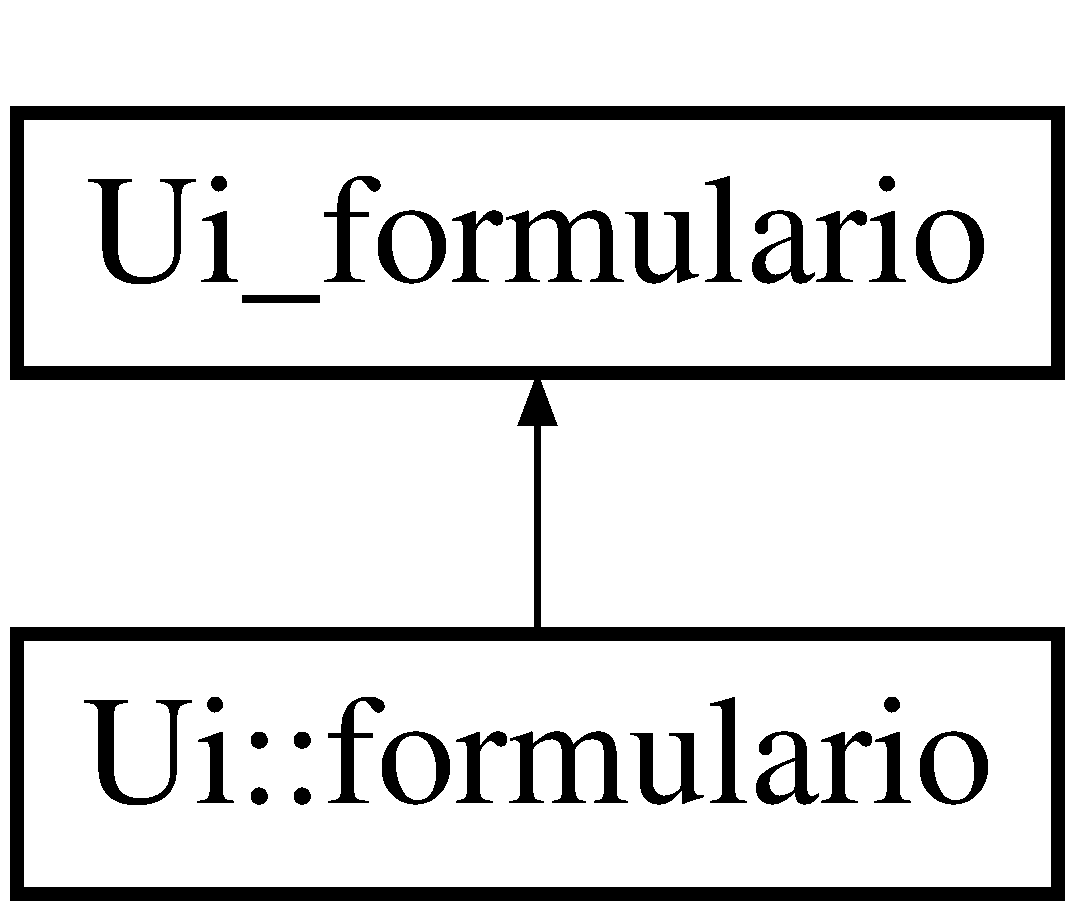
\includegraphics[height=2.000000cm]{class_ui_1_1formulario}
\end{center}
\end{figure}
\subsection*{Additional Inherited Members}


The documentation for this class was generated from the following file\+:\begin{DoxyCompactItemize}
\item 
/home/alseuser/\+Descargas/\+Proyect\+\_\+\+A\+L\+S\+E\+\_\+final/\+Proyect\+\_\+\+A\+L\+S\+E/build/proyecto\+\_\+\+A\+L\+S\+E\+\_\+gui\+\_\+autogen/include/ui\+\_\+formulario.\+h\end{DoxyCompactItemize}

\hypertarget{classformulario}{}\section{formulario Class Reference}
\label{classformulario}\index{formulario@{formulario}}


En esta clase se implementan los métodos usados en la ventana llamada formulario, donde se muestra información del usuario como su edad y el usuario con el que se registró, además, se registran los pacientes de los que se obtiene la información socio económica. luego, se llama la ventana \hyperlink{classmain__app}{main\+\_\+app} en la que se puede realizar la prueba de agilidad.  




{\ttfamily \#include $<$formulario.\+h$>$}

Inheritance diagram for formulario\+:\begin{figure}[H]
\begin{center}
\leavevmode
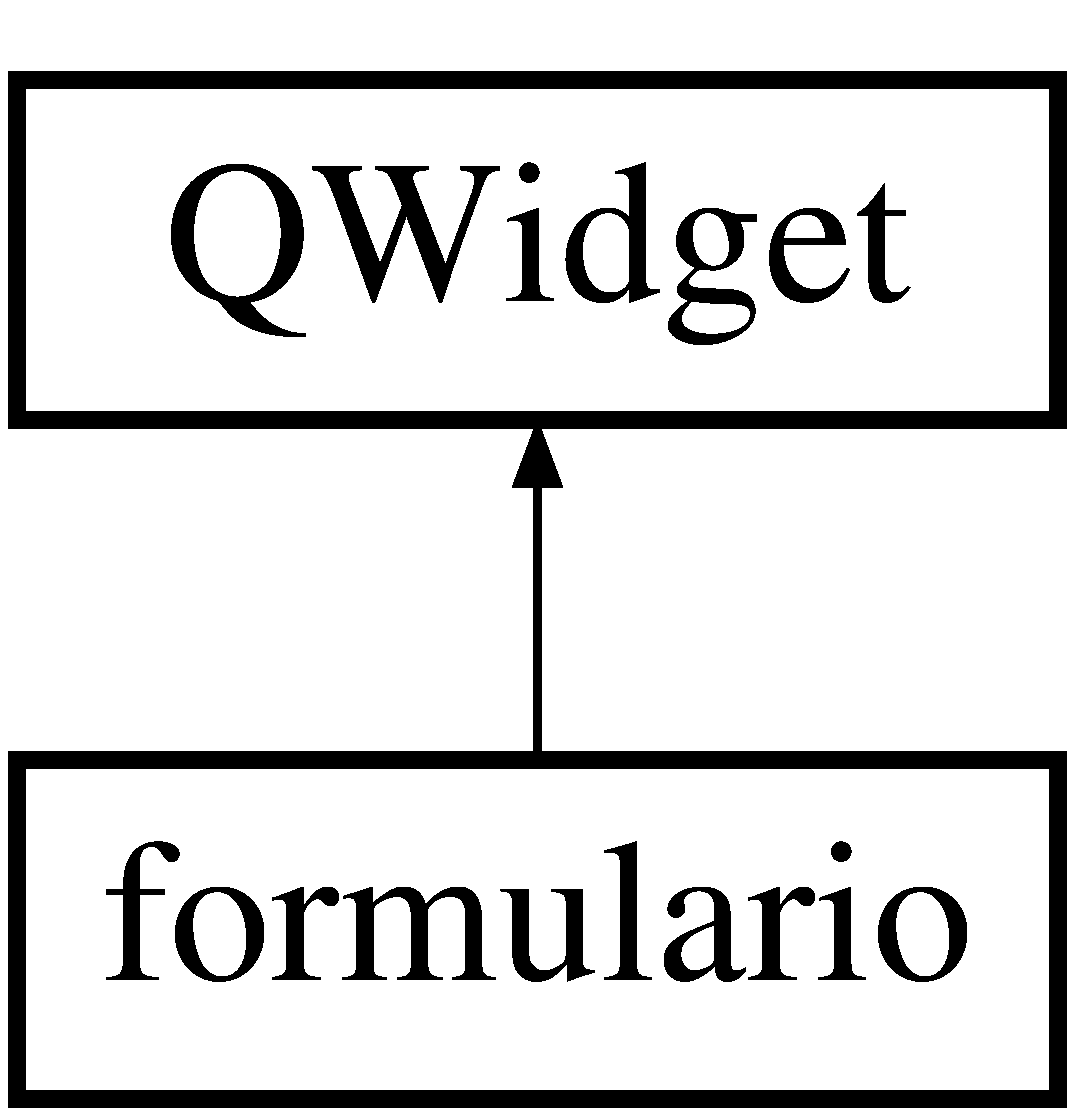
\includegraphics[height=2.000000cm]{classformulario}
\end{center}
\end{figure}
\subsection*{Public Slots}
\begin{DoxyCompactItemize}
\item 
void \hyperlink{classformulario_abf79e0e6729ee886430517ab1159f03e}{recibo\+Datos} (string f, int d)
\end{DoxyCompactItemize}
\subsection*{Signals}
\begin{DoxyCompactItemize}
\item 
\mbox{\Hypertarget{classformulario_a61fdc702dd7c38a8090ed7b2da42d79c}\label{classformulario_a61fdc702dd7c38a8090ed7b2da42d79c}} 
void {\bfseries enviar\+\_\+\+Datostiempo} (int prueba, double cedula\+\_\+paci)
\end{DoxyCompactItemize}
\subsection*{Public Member Functions}
\begin{DoxyCompactItemize}
\item 
\hyperlink{classformulario_af34c9f3ab769a3ea16053537357a8eb2}{formulario} (Q\+Widget $\ast$parent=0)
\item 
\mbox{\Hypertarget{classformulario_ace4314028085911340f58aa6cfcd24ee}\label{classformulario_ace4314028085911340f58aa6cfcd24ee}} 
void {\bfseries set\+\_\+nombreU} (string nombre\+\_\+u)
\item 
\mbox{\Hypertarget{classformulario_a7dcb6cc9155cf10057554d16d399ed12}\label{classformulario_a7dcb6cc9155cf10057554d16d399ed12}} 
string {\bfseries get\+\_\+nombreU} () const
\item 
\mbox{\Hypertarget{classformulario_a8978663040da6ee0a8f2b6add6c25618}\label{classformulario_a8978663040da6ee0a8f2b6add6c25618}} 
void {\bfseries set\+\_\+edad} (int edad)
\item 
\mbox{\Hypertarget{classformulario_a885b709005659b381b5c94d3c1d48f85}\label{classformulario_a885b709005659b381b5c94d3c1d48f85}} 
int {\bfseries get\+\_\+edad} () const
\item 
\mbox{\Hypertarget{classformulario_a26dc6e41c551eaafbfcfa8bec0e69cd6}\label{classformulario_a26dc6e41c551eaafbfcfa8bec0e69cd6}} 
void {\bfseries set\+\_\+tiempoprueba} (int time\+\_\+pru)
\item 
\mbox{\Hypertarget{classformulario_ac78b4c701dd9da8ef7527d5eb69ef95c}\label{classformulario_ac78b4c701dd9da8ef7527d5eb69ef95c}} 
int {\bfseries get\+\_\+tiempoprueba} () const
\item 
\hyperlink{classformulario_a226d2ab871b8816ab3ca146f66e053b4}{$\sim$formulario} ()
\end{DoxyCompactItemize}


\subsection{Detailed Description}
En esta clase se implementan los métodos usados en la ventana llamada formulario, donde se muestra información del usuario como su edad y el usuario con el que se registró, además, se registran los pacientes de los que se obtiene la información socio económica. luego, se llama la ventana \hyperlink{classmain__app}{main\+\_\+app} en la que se puede realizar la prueba de agilidad. 

\subsection{Constructor \& Destructor Documentation}
\mbox{\Hypertarget{classformulario_af34c9f3ab769a3ea16053537357a8eb2}\label{classformulario_af34c9f3ab769a3ea16053537357a8eb2}} 
\index{formulario@{formulario}!formulario@{formulario}}
\index{formulario@{formulario}!formulario@{formulario}}
\subsubsection{\texorpdfstring{formulario()}{formulario()}}
{\footnotesize\ttfamily formulario\+::formulario (\begin{DoxyParamCaption}\item[{Q\+Widget $\ast$}]{parent = {\ttfamily 0} }\end{DoxyParamCaption})\hspace{0.3cm}{\ttfamily [explicit]}}

En esta función se configuran las opciones que pueden salir en las Q\+Widgets llamadas Q\+Combo\+Box, correspondientes a la seleccion de la raza a la que pertenece el paciente o el genero de este. \mbox{\Hypertarget{classformulario_a226d2ab871b8816ab3ca146f66e053b4}\label{classformulario_a226d2ab871b8816ab3ca146f66e053b4}} 
\index{formulario@{formulario}!````~formulario@{$\sim$formulario}}
\index{````~formulario@{$\sim$formulario}!formulario@{formulario}}
\subsubsection{\texorpdfstring{$\sim$formulario()}{~formulario()}}
{\footnotesize\ttfamily formulario\+::$\sim$formulario (\begin{DoxyParamCaption}{ }\end{DoxyParamCaption})}

La funcion detructor nunca puede faltar en una clase, en este caso no ayuda a terminar todo proceso que tenga que ver con la interfaz gráfica de esta ventana. 

\subsection{Member Function Documentation}
\mbox{\Hypertarget{classformulario_abf79e0e6729ee886430517ab1159f03e}\label{classformulario_abf79e0e6729ee886430517ab1159f03e}} 
\index{formulario@{formulario}!recibo\+Datos@{recibo\+Datos}}
\index{recibo\+Datos@{recibo\+Datos}!formulario@{formulario}}
\subsubsection{\texorpdfstring{recibo\+Datos}{reciboDatos}}
{\footnotesize\ttfamily void formulario\+::recibo\+Datos (\begin{DoxyParamCaption}\item[{string}]{f,  }\item[{int}]{d }\end{DoxyParamCaption})\hspace{0.3cm}{\ttfamily [slot]}}

En esta función se reciben el nombre y edad del usuario y se escriben en las Qlabel correspondientes de cada una. 

The documentation for this class was generated from the following files\+:\begin{DoxyCompactItemize}
\item 
/home/alseuser/\+Descargas/\+Proyect\+\_\+\+A\+L\+S\+E\+\_\+final/\+Proyect\+\_\+\+A\+L\+S\+E/formulario.\+h\item 
/home/alseuser/\+Descargas/\+Proyect\+\_\+\+A\+L\+S\+E\+\_\+final/\+Proyect\+\_\+\+A\+L\+S\+E/build/proyecto\+\_\+\+A\+L\+S\+E\+\_\+gui\+\_\+autogen/\+E\+W\+I\+E\+G\+A46\+W\+W/moc\+\_\+formulario.\+cpp\item 
/home/alseuser/\+Descargas/\+Proyect\+\_\+\+A\+L\+S\+E\+\_\+final/\+Proyect\+\_\+\+A\+L\+S\+E/formulario.\+cpp\end{DoxyCompactItemize}

\hypertarget{class_ui_1_1main__app}{}\section{Ui\+:\+:main\+\_\+app Class Reference}
\label{class_ui_1_1main__app}\index{Ui\+::main\+\_\+app@{Ui\+::main\+\_\+app}}
Inheritance diagram for Ui\+:\+:main\+\_\+app\+:\begin{figure}[H]
\begin{center}
\leavevmode
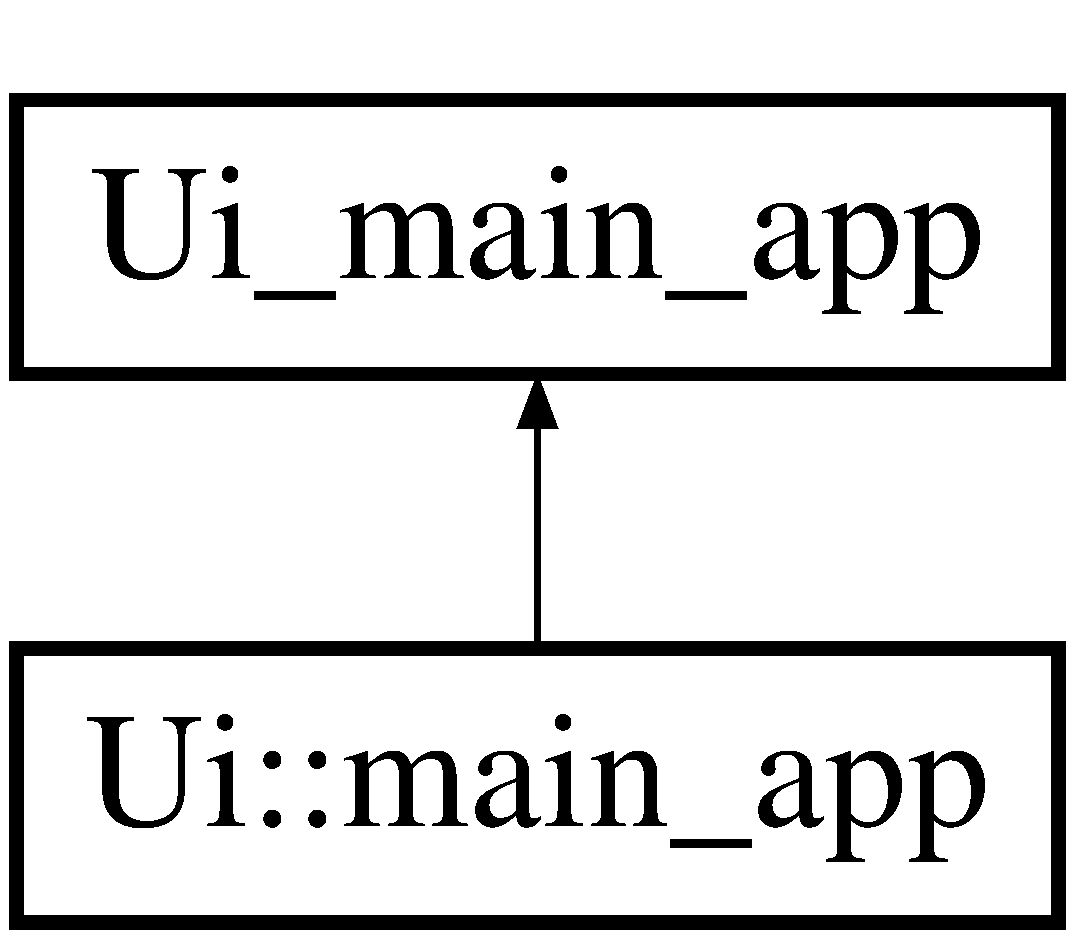
\includegraphics[height=2.000000cm]{class_ui_1_1main__app}
\end{center}
\end{figure}
\subsection*{Additional Inherited Members}


The documentation for this class was generated from the following file\+:\begin{DoxyCompactItemize}
\item 
/home/alseuser/\+Descargas/\+Proyect\+\_\+\+A\+L\+S\+E\+\_\+final/\+Proyect\+\_\+\+A\+L\+S\+E/build/proyecto\+\_\+\+A\+L\+S\+E\+\_\+gui\+\_\+autogen/include/ui\+\_\+main\+\_\+app.\+h\end{DoxyCompactItemize}

\hypertarget{classmain__app}{}\section{main\+\_\+app Class Reference}
\label{classmain__app}\index{main\+\_\+app@{main\+\_\+app}}


En esta clase se va a realizar la prueba de agilidad que debe hacer un paciente al momento de registrarse en nuestro sistema, se guardan en la base de datos el tiempo en el que se oprime un boton especifico, si acerto oprimiendolo y cual paciente este realizando la prueba.  




{\ttfamily \#include $<$main\+\_\+app.\+h$>$}

Inheritance diagram for main\+\_\+app\+:\begin{figure}[H]
\begin{center}
\leavevmode
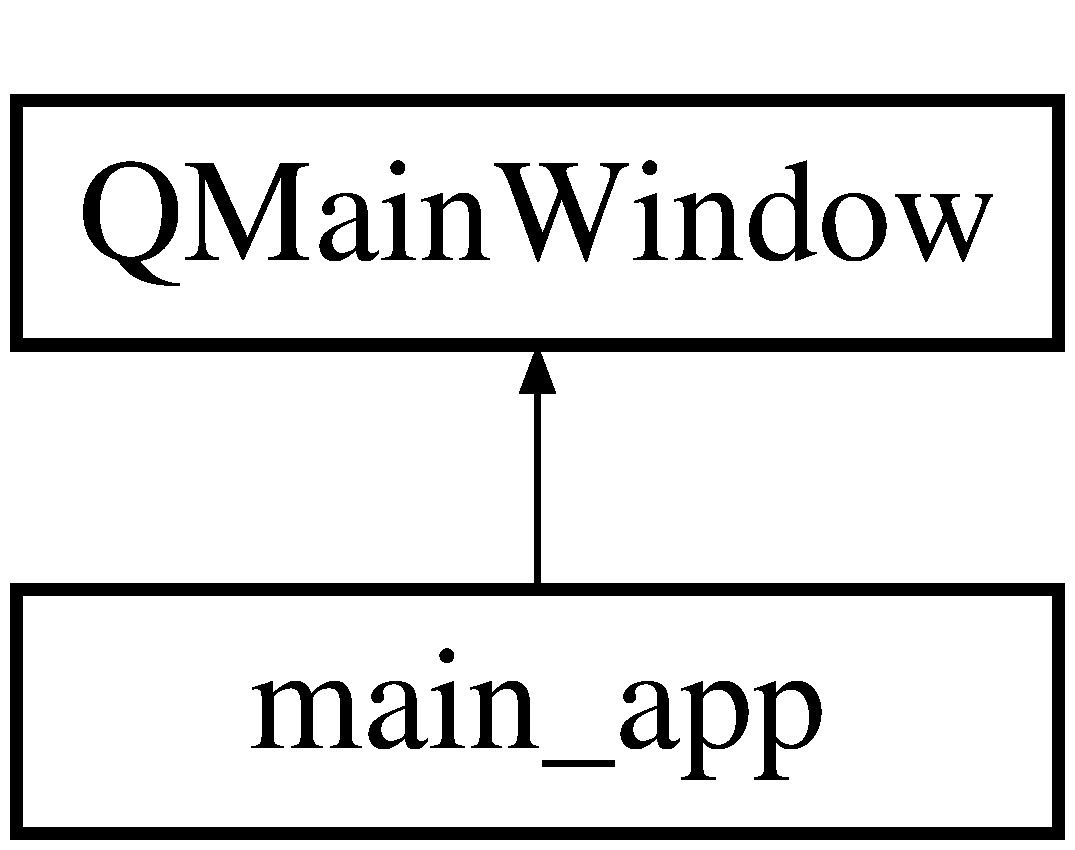
\includegraphics[height=2.000000cm]{classmain__app}
\end{center}
\end{figure}
\subsection*{Public Slots}
\begin{DoxyCompactItemize}
\item 
void \hyperlink{classmain__app_a80f7a386d67024facffb6d1ae66c34d6}{recibo\+\_\+\+Datos} (int time\+\_\+prueba, double pac)
\end{DoxyCompactItemize}
\subsection*{Public Member Functions}
\begin{DoxyCompactItemize}
\item 
\hyperlink{classmain__app_a1d4b63e6e6a588b6d0baf8ad4cc646ce}{main\+\_\+app} (Q\+Widget $\ast$parent=0)
\item 
void \hyperlink{classmain__app_ab7becb80b6053dda9ca04f5ebe774ca0}{Exect} ()
\item 
\hyperlink{classmain__app_af8831d188195a6ac241250985377a7be}{$\sim$main\+\_\+app} ()
\item 
\mbox{\Hypertarget{classmain__app_a1677762bb437a30601c0fa78ba9f043b}\label{classmain__app_a1677762bb437a30601c0fa78ba9f043b}} 
void {\bfseries set\+Tiempo} (int tiempo)
\item 
\mbox{\Hypertarget{classmain__app_a02deefad1525bbabce1fcc372a16e5fe}\label{classmain__app_a02deefad1525bbabce1fcc372a16e5fe}} 
int {\bfseries get\+Tiempo} () const
\item 
\mbox{\Hypertarget{classmain__app_a730cd1902bea7fad2b28eda58c57d8f0}\label{classmain__app_a730cd1902bea7fad2b28eda58c57d8f0}} 
void {\bfseries setcedula} (double cedula)
\item 
\mbox{\Hypertarget{classmain__app_a852eb0ee681b8484ebc036c01f5d5b02}\label{classmain__app_a852eb0ee681b8484ebc036c01f5d5b02}} 
double {\bfseries getcedula} () const
\item 
void \hyperlink{classmain__app_a981265dad144f9c9764c6f263f0dc461}{apagarboton} ()
\item 
void \hyperlink{classmain__app_a2b53dcbe6d60dc8fd978924037ce88cb}{cerrarprueba} ()
\end{DoxyCompactItemize}
\subsection*{Public Attributes}
\begin{DoxyCompactItemize}
\item 
\mbox{\Hypertarget{classmain__app_a0b65200fbc076026b07434b395500268}\label{classmain__app_a0b65200fbc076026b07434b395500268}} 
Q\+Timer $\ast$ {\bfseries tiempo\+\_\+prueba}
\end{DoxyCompactItemize}


\subsection{Detailed Description}
En esta clase se va a realizar la prueba de agilidad que debe hacer un paciente al momento de registrarse en nuestro sistema, se guardan en la base de datos el tiempo en el que se oprime un boton especifico, si acerto oprimiendolo y cual paciente este realizando la prueba. 

\subsection{Constructor \& Destructor Documentation}
\mbox{\Hypertarget{classmain__app_a1d4b63e6e6a588b6d0baf8ad4cc646ce}\label{classmain__app_a1d4b63e6e6a588b6d0baf8ad4cc646ce}} 
\index{main\+\_\+app@{main\+\_\+app}!main\+\_\+app@{main\+\_\+app}}
\index{main\+\_\+app@{main\+\_\+app}!main\+\_\+app@{main\+\_\+app}}
\subsubsection{\texorpdfstring{main\+\_\+app()}{main\_app()}}
{\footnotesize\ttfamily main\+\_\+app\+::main\+\_\+app (\begin{DoxyParamCaption}\item[{Q\+Widget $\ast$}]{parent = {\ttfamily 0} }\end{DoxyParamCaption})\hspace{0.3cm}{\ttfamily [explicit]}}

En esta función configuramos el tamaño, color y figura de los botones que se van a usar para la prueba de agilidad del paciente, además, se realizan los connect que reciben las instrucciones emitidas por la funcion timeout de la clase Qtimer, que son los \char`\"{}contadores\char`\"{} usados para el cambio de estados en cada botón. \mbox{\Hypertarget{classmain__app_af8831d188195a6ac241250985377a7be}\label{classmain__app_af8831d188195a6ac241250985377a7be}} 
\index{main\+\_\+app@{main\+\_\+app}!````~main\+\_\+app@{$\sim$main\+\_\+app}}
\index{````~main\+\_\+app@{$\sim$main\+\_\+app}!main\+\_\+app@{main\+\_\+app}}
\subsubsection{\texorpdfstring{$\sim$main\+\_\+app()}{~main\_app()}}
{\footnotesize\ttfamily main\+\_\+app\+::$\sim$main\+\_\+app (\begin{DoxyParamCaption}{ }\end{DoxyParamCaption})}

El destructor de la clase, llamado cuando se acaben las instrucciones relacionadas con esta clase. 

\subsection{Member Function Documentation}
\mbox{\Hypertarget{classmain__app_a981265dad144f9c9764c6f263f0dc461}\label{classmain__app_a981265dad144f9c9764c6f263f0dc461}} 
\index{main\+\_\+app@{main\+\_\+app}!apagarboton@{apagarboton}}
\index{apagarboton@{apagarboton}!main\+\_\+app@{main\+\_\+app}}
\subsubsection{\texorpdfstring{apagarboton()}{apagarboton()}}
{\footnotesize\ttfamily void main\+\_\+app\+::apagarboton (\begin{DoxyParamCaption}{ }\end{DoxyParamCaption})}

Esta función manda la información del paciente, el tiempo en el que se oprimió un botón, cual boton oprimió y si era el correcto. Además, escoge al azar un valor entre 1 y 11 para hacer que la prueba sea totalmente aleatoria y no se repita ningún ciclo en los botones. \mbox{\Hypertarget{classmain__app_a2b53dcbe6d60dc8fd978924037ce88cb}\label{classmain__app_a2b53dcbe6d60dc8fd978924037ce88cb}} 
\index{main\+\_\+app@{main\+\_\+app}!cerrarprueba@{cerrarprueba}}
\index{cerrarprueba@{cerrarprueba}!main\+\_\+app@{main\+\_\+app}}
\subsubsection{\texorpdfstring{cerrarprueba()}{cerrarprueba()}}
{\footnotesize\ttfamily void main\+\_\+app\+::cerrarprueba (\begin{DoxyParamCaption}{ }\end{DoxyParamCaption})}

Al momento de acabar el tiempo al que se configuró la prueba, se llama a esta función para cerrar la base de datos y cerrar la ventana tambien. \mbox{\Hypertarget{classmain__app_ab7becb80b6053dda9ca04f5ebe774ca0}\label{classmain__app_ab7becb80b6053dda9ca04f5ebe774ca0}} 
\index{main\+\_\+app@{main\+\_\+app}!Exect@{Exect}}
\index{Exect@{Exect}!main\+\_\+app@{main\+\_\+app}}
\subsubsection{\texorpdfstring{Exect()}{Exect()}}
{\footnotesize\ttfamily void main\+\_\+app\+::\+Exect (\begin{DoxyParamCaption}{ }\end{DoxyParamCaption})}

Esta función vuelve visible la ventana en la que ingresa un usuario a la plataforma de registros, además, la vuelve modal. \mbox{\Hypertarget{classmain__app_a80f7a386d67024facffb6d1ae66c34d6}\label{classmain__app_a80f7a386d67024facffb6d1ae66c34d6}} 
\index{main\+\_\+app@{main\+\_\+app}!recibo\+\_\+\+Datos@{recibo\+\_\+\+Datos}}
\index{recibo\+\_\+\+Datos@{recibo\+\_\+\+Datos}!main\+\_\+app@{main\+\_\+app}}
\subsubsection{\texorpdfstring{recibo\+\_\+\+Datos}{recibo\_Datos}}
{\footnotesize\ttfamily void main\+\_\+app\+::recibo\+\_\+\+Datos (\begin{DoxyParamCaption}\item[{int}]{time\+\_\+prueba,  }\item[{double}]{pac }\end{DoxyParamCaption})\hspace{0.3cm}{\ttfamily [slot]}}

Esta función recibe los datos del documento del paciente que realizara la prueba y el tiempo que va a durar realizando esta misma. 

The documentation for this class was generated from the following files\+:\begin{DoxyCompactItemize}
\item 
/home/alseuser/\+Descargas/\+Proyect\+\_\+\+A\+L\+S\+E\+\_\+final/\+Proyect\+\_\+\+A\+L\+S\+E/main\+\_\+app.\+h\item 
/home/alseuser/\+Descargas/\+Proyect\+\_\+\+A\+L\+S\+E\+\_\+final/\+Proyect\+\_\+\+A\+L\+S\+E/main\+\_\+app.\+cpp\end{DoxyCompactItemize}

\hypertarget{classpaciente}{}\section{paciente Class Reference}
\label{classpaciente}\index{paciente@{paciente}}


En esta clase definimos la información básica que debe tener un paciente, implementando las funciones Getter y Setter como funciones inline que permiten un mejor funcionamiento del programa.  




{\ttfamily \#include $<$paciente.\+h$>$}

\subsection*{Public Member Functions}
\begin{DoxyCompactItemize}
\item 
\hyperlink{classpaciente_ac81d0605801b88c3b9e10d828730240d}{paciente} ()
\item 
\mbox{\Hypertarget{classpaciente_a9fcf7f5f18047a4410d6d180cfae3f28}\label{classpaciente_a9fcf7f5f18047a4410d6d180cfae3f28}} 
void {\bfseries set\+Fecha} (string fecha)
\item 
\mbox{\Hypertarget{classpaciente_a26d230b5ce526b9036dc99fed96cda6c}\label{classpaciente_a26d230b5ce526b9036dc99fed96cda6c}} 
string {\bfseries get\+Fecha} () const
\item 
\mbox{\Hypertarget{classpaciente_ab74e3d7bf42aecc8585729823442a229}\label{classpaciente_ab74e3d7bf42aecc8585729823442a229}} 
void {\bfseries set\+Doc} (double Doc)
\item 
\mbox{\Hypertarget{classpaciente_afcc011800582077e90de55a7e273a0f5}\label{classpaciente_afcc011800582077e90de55a7e273a0f5}} 
double {\bfseries get\+Doc} () const
\item 
\mbox{\Hypertarget{classpaciente_ad0b05ef2dd5e5789569a6876218b18e6}\label{classpaciente_ad0b05ef2dd5e5789569a6876218b18e6}} 
void {\bfseries set\+Nombre} (string nombre)
\item 
\mbox{\Hypertarget{classpaciente_ade5b611666a067d54d8cee91bf737f2a}\label{classpaciente_ade5b611666a067d54d8cee91bf737f2a}} 
string {\bfseries get\+Nombre} () const
\item 
\mbox{\Hypertarget{classpaciente_a8738238cef3427afe0bfd2c638a524d5}\label{classpaciente_a8738238cef3427afe0bfd2c638a524d5}} 
void {\bfseries set\+Apellido} (string apellido)
\item 
\mbox{\Hypertarget{classpaciente_acc71b2d1b5654d36f55c584024f0b647}\label{classpaciente_acc71b2d1b5654d36f55c584024f0b647}} 
string {\bfseries get\+Apellido} () const
\item 
\mbox{\Hypertarget{classpaciente_a26d57e3fa8d416751d1809312471793a}\label{classpaciente_a26d57e3fa8d416751d1809312471793a}} 
void {\bfseries set\+Raza} (string raza)
\item 
\mbox{\Hypertarget{classpaciente_a45a970e862620174070e467ef1f459cb}\label{classpaciente_a45a970e862620174070e467ef1f459cb}} 
string {\bfseries get\+Raza} () const
\item 
\mbox{\Hypertarget{classpaciente_a5b53736726dde5ab654228184b078f05}\label{classpaciente_a5b53736726dde5ab654228184b078f05}} 
void {\bfseries set\+Genero} (string genero)
\item 
\mbox{\Hypertarget{classpaciente_a51e493163e84062d8ee70b545fff298a}\label{classpaciente_a51e493163e84062d8ee70b545fff298a}} 
string {\bfseries get\+Genero} () const
\item 
\mbox{\Hypertarget{classpaciente_a4ce7ba7647d1d12bac4620385b256cad}\label{classpaciente_a4ce7ba7647d1d12bac4620385b256cad}} 
void {\bfseries set\+Ingreso} (double ingreso)
\item 
\mbox{\Hypertarget{classpaciente_a0446f2e504093bbce1a6e80a21a6b986}\label{classpaciente_a0446f2e504093bbce1a6e80a21a6b986}} 
double {\bfseries get\+Ingreso} () const
\item 
\mbox{\Hypertarget{classpaciente_a6d93e288ff755fc5bd1c433b9f3f6de2}\label{classpaciente_a6d93e288ff755fc5bd1c433b9f3f6de2}} 
void {\bfseries set\+Direccion} (string direccion)
\item 
\mbox{\Hypertarget{classpaciente_a66e228c19e21057d1d683e2c44f1ff88}\label{classpaciente_a66e228c19e21057d1d683e2c44f1ff88}} 
string {\bfseries get\+Direccion} () const
\end{DoxyCompactItemize}


\subsection{Detailed Description}
En esta clase definimos la información básica que debe tener un paciente, implementando las funciones Getter y Setter como funciones inline que permiten un mejor funcionamiento del programa. 

\subsection{Constructor \& Destructor Documentation}
\mbox{\Hypertarget{classpaciente_ac81d0605801b88c3b9e10d828730240d}\label{classpaciente_ac81d0605801b88c3b9e10d828730240d}} 
\index{paciente@{paciente}!paciente@{paciente}}
\index{paciente@{paciente}!paciente@{paciente}}
\subsubsection{\texorpdfstring{paciente()}{paciente()}}
{\footnotesize\ttfamily paciente\+::paciente (\begin{DoxyParamCaption}{ }\end{DoxyParamCaption})}

La implementación de esta clase no es necesaria ya que hicimos uso de funciones inline. 

The documentation for this class was generated from the following files\+:\begin{DoxyCompactItemize}
\item 
/home/alseuser/\+Descargas/\+Proyect\+\_\+\+A\+L\+S\+E\+\_\+final/\+Proyect\+\_\+\+A\+L\+S\+E/paciente.\+h\item 
/home/alseuser/\+Descargas/\+Proyect\+\_\+\+A\+L\+S\+E\+\_\+final/\+Proyect\+\_\+\+A\+L\+S\+E/paciente.\+cpp\end{DoxyCompactItemize}

\hypertarget{classplataforma}{}\section{plataforma Class Reference}
\label{classplataforma}\index{plataforma@{plataforma}}


Una ventana de esta clase es la que inicia el sistema de todo el programa, pues es donde se registra e ingresa un usuario. Es quien llama a las ventanas registro y formulario.  




{\ttfamily \#include $<$plataforma.\+h$>$}

Inheritance diagram for plataforma\+:\begin{figure}[H]
\begin{center}
\leavevmode
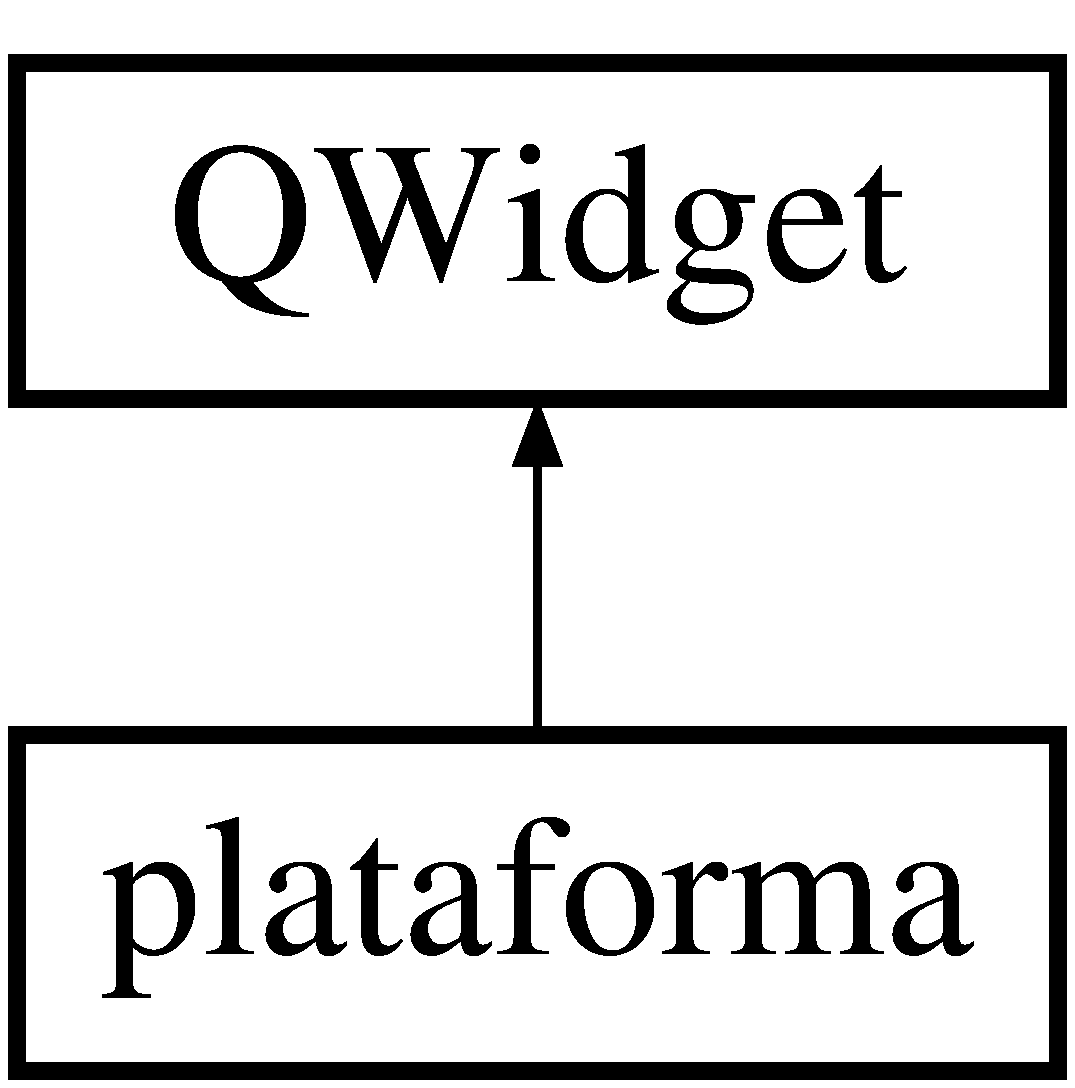
\includegraphics[height=2.000000cm]{classplataforma}
\end{center}
\end{figure}
\subsection*{Signals}
\begin{DoxyCompactItemize}
\item 
\mbox{\Hypertarget{classplataforma_a7059858bf747f452aff90d1486bad552}\label{classplataforma_a7059858bf747f452aff90d1486bad552}} 
void {\bfseries enviar\+Datos} (string first, int divisor)
\end{DoxyCompactItemize}
\subsection*{Public Member Functions}
\begin{DoxyCompactItemize}
\item 
\hyperlink{classplataforma_a200eafd497e5192ed3c535ad9653d824}{plataforma} (Q\+Widget $\ast$parent=0)
\item 
\hyperlink{classplataforma_a8c90e738adb0469626698000d7760c85}{$\sim$plataforma} ()
\item 
\mbox{\Hypertarget{classplataforma_a59714e2d864f14e52c8d79643c9909da}\label{classplataforma_a59714e2d864f14e52c8d79643c9909da}} 
void {\bfseries set\+\_\+nombreU} (string nombre\+\_\+u)
\item 
\mbox{\Hypertarget{classplataforma_a8bb7f8ccc1cceedbaab2b8b1670ead63}\label{classplataforma_a8bb7f8ccc1cceedbaab2b8b1670ead63}} 
string {\bfseries get\+\_\+nombreU} () const
\item 
\mbox{\Hypertarget{classplataforma_a409b831a0f70bd38137f37519de3835a}\label{classplataforma_a409b831a0f70bd38137f37519de3835a}} 
void {\bfseries set\+\_\+edadU} (int edad)
\item 
\mbox{\Hypertarget{classplataforma_a669292aaf311df5ac54d948c9985eed8}\label{classplataforma_a669292aaf311df5ac54d948c9985eed8}} 
int {\bfseries get\+\_\+edadU} () const
\end{DoxyCompactItemize}


\subsection{Detailed Description}
Una ventana de esta clase es la que inicia el sistema de todo el programa, pues es donde se registra e ingresa un usuario. Es quien llama a las ventanas registro y formulario. 

\subsection{Constructor \& Destructor Documentation}
\mbox{\Hypertarget{classplataforma_a200eafd497e5192ed3c535ad9653d824}\label{classplataforma_a200eafd497e5192ed3c535ad9653d824}} 
\index{plataforma@{plataforma}!plataforma@{plataforma}}
\index{plataforma@{plataforma}!plataforma@{plataforma}}
\subsubsection{\texorpdfstring{plataforma()}{plataforma()}}
{\footnotesize\ttfamily plataforma\+::plataforma (\begin{DoxyParamCaption}\item[{Q\+Widget $\ast$}]{parent = {\ttfamily 0} }\end{DoxyParamCaption})\hspace{0.3cm}{\ttfamily [explicit]}}

Esta funcion inicializa los procesos que se vayan a realizar en la G\+UI de esta clase. \mbox{\Hypertarget{classplataforma_a8c90e738adb0469626698000d7760c85}\label{classplataforma_a8c90e738adb0469626698000d7760c85}} 
\index{plataforma@{plataforma}!````~plataforma@{$\sim$plataforma}}
\index{````~plataforma@{$\sim$plataforma}!plataforma@{plataforma}}
\subsubsection{\texorpdfstring{$\sim$plataforma()}{~plataforma()}}
{\footnotesize\ttfamily plataforma\+::$\sim$plataforma (\begin{DoxyParamCaption}{ }\end{DoxyParamCaption})}

El destructor de esta clase destruye todas las variables que se hayan usado en algún proceso que realice una función y ya no sea necesaria. Libera recursos. 

The documentation for this class was generated from the following files\+:\begin{DoxyCompactItemize}
\item 
/home/alseuser/\+Descargas/\+Proyect\+\_\+\+A\+L\+S\+E\+\_\+final/\+Proyect\+\_\+\+A\+L\+S\+E/plataforma.\+h\item 
/home/alseuser/\+Descargas/\+Proyect\+\_\+\+A\+L\+S\+E\+\_\+final/\+Proyect\+\_\+\+A\+L\+S\+E/build/proyecto\+\_\+\+A\+L\+S\+E\+\_\+gui\+\_\+autogen/\+E\+W\+I\+E\+G\+A46\+W\+W/moc\+\_\+plataforma.\+cpp\item 
/home/alseuser/\+Descargas/\+Proyect\+\_\+\+A\+L\+S\+E\+\_\+final/\+Proyect\+\_\+\+A\+L\+S\+E/plataforma.\+cpp\end{DoxyCompactItemize}

\hypertarget{class_ui_1_1plataforma}{}\section{Ui\+:\+:plataforma Class Reference}
\label{class_ui_1_1plataforma}\index{Ui\+::plataforma@{Ui\+::plataforma}}
Inheritance diagram for Ui\+:\+:plataforma\+:\begin{figure}[H]
\begin{center}
\leavevmode
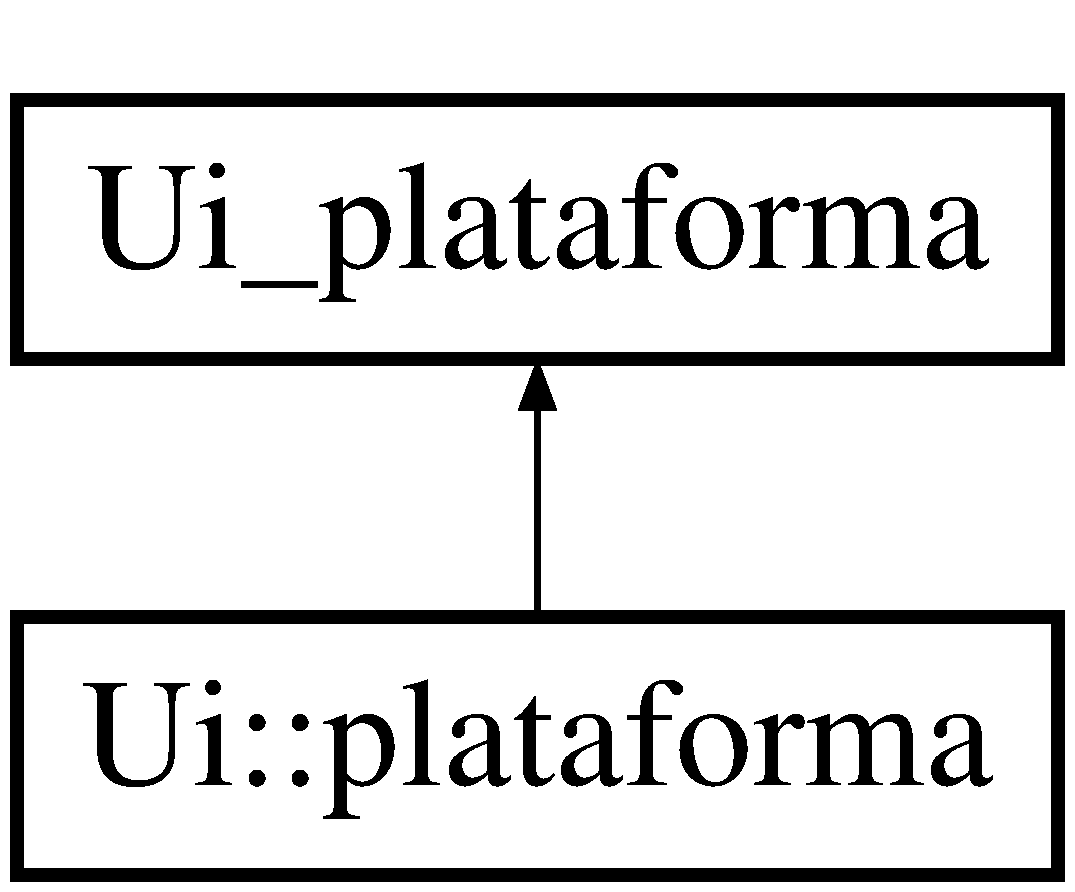
\includegraphics[height=2.000000cm]{class_ui_1_1plataforma}
\end{center}
\end{figure}
\subsection*{Additional Inherited Members}


The documentation for this class was generated from the following file\+:\begin{DoxyCompactItemize}
\item 
/home/alseuser/\+Descargas/\+Proyect\+\_\+\+A\+L\+S\+E\+\_\+final/\+Proyect\+\_\+\+A\+L\+S\+E/build/proyecto\+\_\+\+A\+L\+S\+E\+\_\+gui\+\_\+autogen/include/ui\+\_\+plataforma.\+h\end{DoxyCompactItemize}

\hypertarget{structqt__meta__stringdata__formulario__t}{}\section{qt\+\_\+meta\+\_\+stringdata\+\_\+formulario\+\_\+t Struct Reference}
\label{structqt__meta__stringdata__formulario__t}\index{qt\+\_\+meta\+\_\+stringdata\+\_\+formulario\+\_\+t@{qt\+\_\+meta\+\_\+stringdata\+\_\+formulario\+\_\+t}}
\subsection*{Public Attributes}
\begin{DoxyCompactItemize}
\item 
\mbox{\Hypertarget{structqt__meta__stringdata__formulario__t_a16064cc2d54827c3ccad21ef7e5f33cb}\label{structqt__meta__stringdata__formulario__t_a16064cc2d54827c3ccad21ef7e5f33cb}} 
Q\+Byte\+Array\+Data {\bfseries data} \mbox{[}21\mbox{]}
\item 
\mbox{\Hypertarget{structqt__meta__stringdata__formulario__t_a69f9ddfd6de21fe6e0fe7e5869e622a9}\label{structqt__meta__stringdata__formulario__t_a69f9ddfd6de21fe6e0fe7e5869e622a9}} 
char {\bfseries stringdata0} \mbox{[}319\mbox{]}
\end{DoxyCompactItemize}


The documentation for this struct was generated from the following file\+:\begin{DoxyCompactItemize}
\item 
/home/alseuser/\+Descargas/\+Proyect\+\_\+\+A\+L\+S\+E\+\_\+final/\+Proyect\+\_\+\+A\+L\+S\+E/build/proyecto\+\_\+\+A\+L\+S\+E\+\_\+gui\+\_\+autogen/\+E\+W\+I\+E\+G\+A46\+W\+W/moc\+\_\+formulario.\+cpp\end{DoxyCompactItemize}

\hypertarget{structqt__meta__stringdata__main__app__t}{}\section{qt\+\_\+meta\+\_\+stringdata\+\_\+main\+\_\+app\+\_\+t Struct Reference}
\label{structqt__meta__stringdata__main__app__t}\index{qt\+\_\+meta\+\_\+stringdata\+\_\+main\+\_\+app\+\_\+t@{qt\+\_\+meta\+\_\+stringdata\+\_\+main\+\_\+app\+\_\+t}}
\subsection*{Public Attributes}
\begin{DoxyCompactItemize}
\item 
\mbox{\Hypertarget{structqt__meta__stringdata__main__app__t_a2542dda2913bba59b7d8e2ec9beb0200}\label{structqt__meta__stringdata__main__app__t_a2542dda2913bba59b7d8e2ec9beb0200}} 
Q\+Byte\+Array\+Data {\bfseries data} \mbox{[}18\mbox{]}
\item 
\mbox{\Hypertarget{structqt__meta__stringdata__main__app__t_a361fe627da7674ae842bdb04cbbc6ee6}\label{structqt__meta__stringdata__main__app__t_a361fe627da7674ae842bdb04cbbc6ee6}} 
char {\bfseries stringdata0} \mbox{[}229\mbox{]}
\end{DoxyCompactItemize}


The documentation for this struct was generated from the following file\+:\begin{DoxyCompactItemize}
\item 
/home/alseuser/\+Descargas/\+Proyect\+\_\+\+A\+L\+S\+E\+\_\+final/\+Proyect\+\_\+\+A\+L\+S\+E/build/proyecto\+\_\+\+A\+L\+S\+E\+\_\+gui\+\_\+autogen/\+E\+W\+I\+E\+G\+A46\+W\+W/moc\+\_\+main\+\_\+app.\+cpp\end{DoxyCompactItemize}

\hypertarget{structqt__meta__stringdata__plataforma__t}{}\section{qt\+\_\+meta\+\_\+stringdata\+\_\+plataforma\+\_\+t Struct Reference}
\label{structqt__meta__stringdata__plataforma__t}\index{qt\+\_\+meta\+\_\+stringdata\+\_\+plataforma\+\_\+t@{qt\+\_\+meta\+\_\+stringdata\+\_\+plataforma\+\_\+t}}
\subsection*{Public Attributes}
\begin{DoxyCompactItemize}
\item 
\mbox{\Hypertarget{structqt__meta__stringdata__plataforma__t_a750e6298fb768b251d0b1ba37e969bb5}\label{structqt__meta__stringdata__plataforma__t_a750e6298fb768b251d0b1ba37e969bb5}} 
Q\+Byte\+Array\+Data {\bfseries data} \mbox{[}8\mbox{]}
\item 
\mbox{\Hypertarget{structqt__meta__stringdata__plataforma__t_a13cb93df2af9ade9b2f2a4b1f9a78d65}\label{structqt__meta__stringdata__plataforma__t_a13cb93df2af9ade9b2f2a4b1f9a78d65}} 
char {\bfseries stringdata0} \mbox{[}88\mbox{]}
\end{DoxyCompactItemize}


The documentation for this struct was generated from the following file\+:\begin{DoxyCompactItemize}
\item 
/home/alseuser/\+Descargas/\+Proyect\+\_\+\+A\+L\+S\+E\+\_\+final/\+Proyect\+\_\+\+A\+L\+S\+E/build/proyecto\+\_\+\+A\+L\+S\+E\+\_\+gui\+\_\+autogen/\+E\+W\+I\+E\+G\+A46\+W\+W/moc\+\_\+plataforma.\+cpp\end{DoxyCompactItemize}

\hypertarget{structqt__meta__stringdata__registro__t}{}\section{qt\+\_\+meta\+\_\+stringdata\+\_\+registro\+\_\+t Struct Reference}
\label{structqt__meta__stringdata__registro__t}\index{qt\+\_\+meta\+\_\+stringdata\+\_\+registro\+\_\+t@{qt\+\_\+meta\+\_\+stringdata\+\_\+registro\+\_\+t}}
\subsection*{Public Attributes}
\begin{DoxyCompactItemize}
\item 
\mbox{\Hypertarget{structqt__meta__stringdata__registro__t_aabfb527b208296c0a72b076bb0d223ed}\label{structqt__meta__stringdata__registro__t_aabfb527b208296c0a72b076bb0d223ed}} 
Q\+Byte\+Array\+Data {\bfseries data} \mbox{[}10\mbox{]}
\item 
\mbox{\Hypertarget{structqt__meta__stringdata__registro__t_a07e00c83aed576505de5b2b4294a8cea}\label{structqt__meta__stringdata__registro__t_a07e00c83aed576505de5b2b4294a8cea}} 
char {\bfseries stringdata0} \mbox{[}182\mbox{]}
\end{DoxyCompactItemize}


The documentation for this struct was generated from the following file\+:\begin{DoxyCompactItemize}
\item 
/home/alseuser/\+Descargas/\+Proyect\+\_\+\+A\+L\+S\+E\+\_\+final/\+Proyect\+\_\+\+A\+L\+S\+E/build/proyecto\+\_\+\+A\+L\+S\+E\+\_\+gui\+\_\+autogen/\+E\+W\+I\+E\+G\+A46\+W\+W/moc\+\_\+registro.\+cpp\end{DoxyCompactItemize}

\hypertarget{classregistro}{}\section{registro Class Reference}
\label{classregistro}\index{registro@{registro}}


Esta clase es la responsable de registrar un usuario en el sistema y de guardar sus datos básicos, verificando que su cédula no se haya registrado anteriormente, en el caso que se encuentre esta cédula en la base de datos se le informará de este error por medio de la G\+UI.  




{\ttfamily \#include $<$registro.\+h$>$}

Inheritance diagram for registro\+:\begin{figure}[H]
\begin{center}
\leavevmode
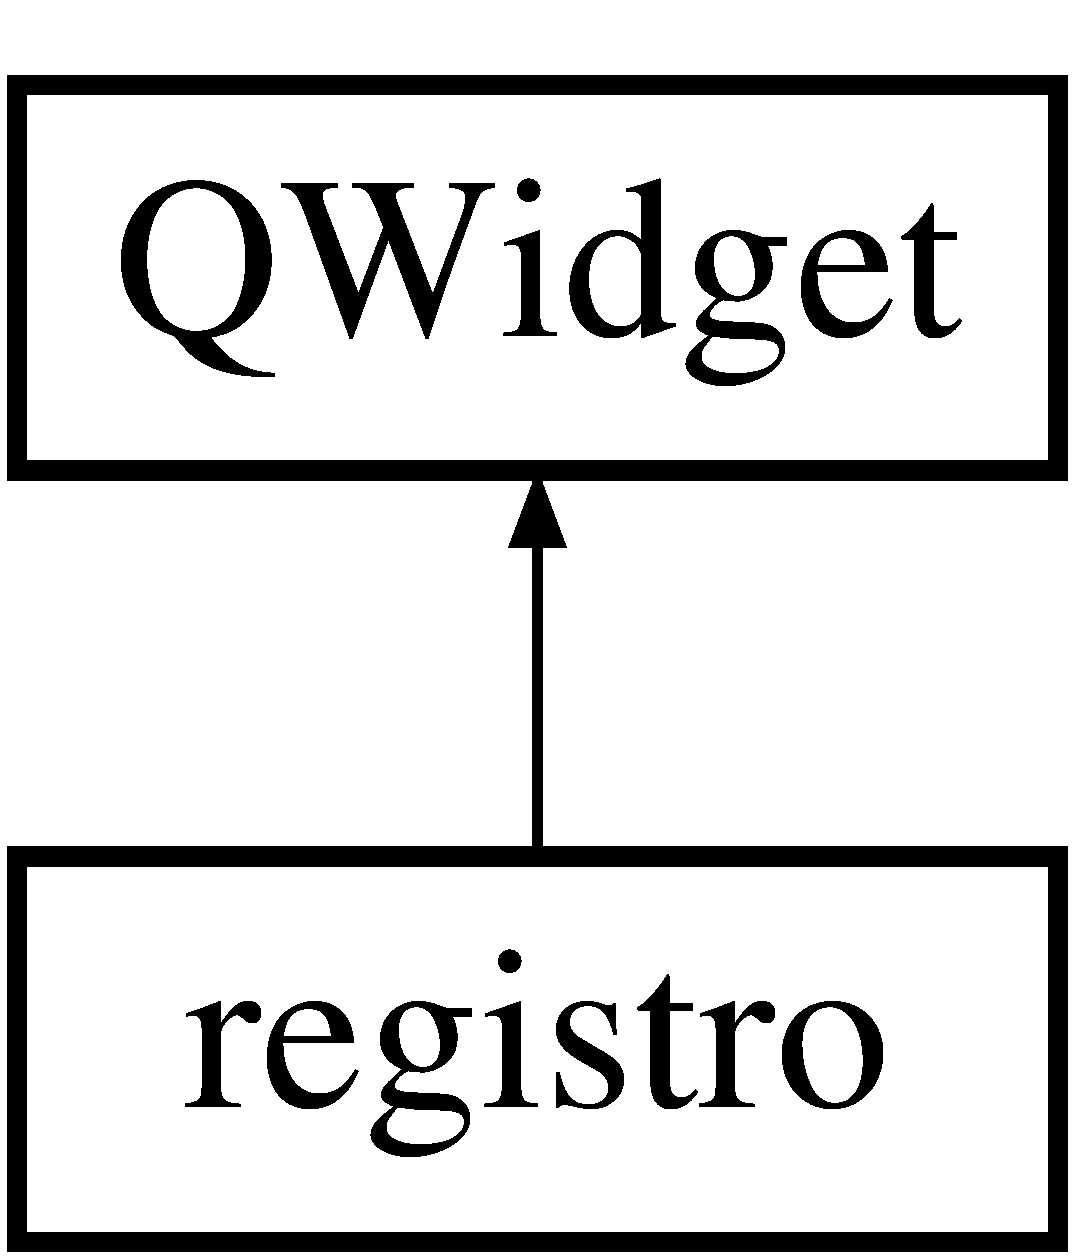
\includegraphics[height=2.000000cm]{classregistro}
\end{center}
\end{figure}
\subsection*{Public Member Functions}
\begin{DoxyCompactItemize}
\item 
\hyperlink{classregistro_a1603a3ccdbb5e4fb01ba21158e3f8dfa}{registro} (Q\+Widget $\ast$parent=0)
\item 
\hyperlink{classregistro_addf760db779d168a84ef54c49ada3c74}{$\sim$registro} ()
\end{DoxyCompactItemize}


\subsection{Detailed Description}
Esta clase es la responsable de registrar un usuario en el sistema y de guardar sus datos básicos, verificando que su cédula no se haya registrado anteriormente, en el caso que se encuentre esta cédula en la base de datos se le informará de este error por medio de la G\+UI. 

\subsection{Constructor \& Destructor Documentation}
\mbox{\Hypertarget{classregistro_a1603a3ccdbb5e4fb01ba21158e3f8dfa}\label{classregistro_a1603a3ccdbb5e4fb01ba21158e3f8dfa}} 
\index{registro@{registro}!registro@{registro}}
\index{registro@{registro}!registro@{registro}}
\subsubsection{\texorpdfstring{registro()}{registro()}}
{\footnotesize\ttfamily registro\+::registro (\begin{DoxyParamCaption}\item[{Q\+Widget $\ast$}]{parent = {\ttfamily 0} }\end{DoxyParamCaption})\hspace{0.3cm}{\ttfamily [explicit]}}

Esta función inicializa los procesos que se van a realizar con esta clase. \mbox{\Hypertarget{classregistro_addf760db779d168a84ef54c49ada3c74}\label{classregistro_addf760db779d168a84ef54c49ada3c74}} 
\index{registro@{registro}!````~registro@{$\sim$registro}}
\index{````~registro@{$\sim$registro}!registro@{registro}}
\subsubsection{\texorpdfstring{$\sim$registro()}{~registro()}}
{\footnotesize\ttfamily registro\+::$\sim$registro (\begin{DoxyParamCaption}{ }\end{DoxyParamCaption})}

El destructor de una clase elimina las variables temporales que se hayan usado para hacer algún calculo y que ya no se necesiten. 

The documentation for this class was generated from the following files\+:\begin{DoxyCompactItemize}
\item 
/home/alseuser/\+Descargas/\+Proyect\+\_\+\+A\+L\+S\+E\+\_\+final/\+Proyect\+\_\+\+A\+L\+S\+E/registro.\+h\item 
/home/alseuser/\+Descargas/\+Proyect\+\_\+\+A\+L\+S\+E\+\_\+final/\+Proyect\+\_\+\+A\+L\+S\+E/registro.\+cpp\end{DoxyCompactItemize}

\hypertarget{class_ui_1_1registro}{}\section{Ui\+:\+:registro Class Reference}
\label{class_ui_1_1registro}\index{Ui\+::registro@{Ui\+::registro}}
Inheritance diagram for Ui\+:\+:registro\+:\begin{figure}[H]
\begin{center}
\leavevmode
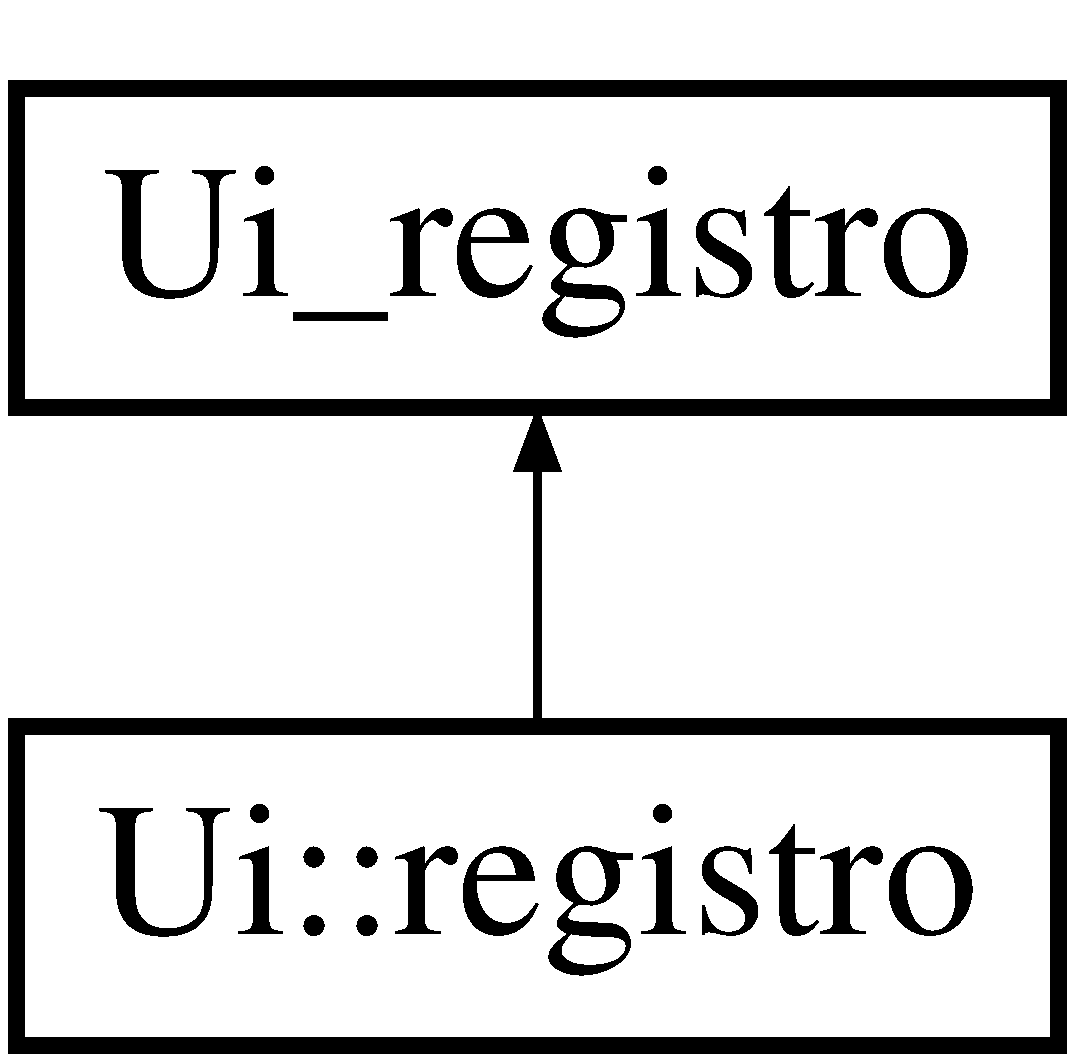
\includegraphics[height=2.000000cm]{class_ui_1_1registro}
\end{center}
\end{figure}
\subsection*{Additional Inherited Members}


The documentation for this class was generated from the following file\+:\begin{DoxyCompactItemize}
\item 
/home/alseuser/\+Descargas/\+Proyect\+\_\+\+A\+L\+S\+E\+\_\+final/\+Proyect\+\_\+\+A\+L\+S\+E/build/proyecto\+\_\+\+A\+L\+S\+E\+\_\+gui\+\_\+autogen/include/ui\+\_\+registro.\+h\end{DoxyCompactItemize}

\hypertarget{class_ui__formulario}{}\section{Ui\+\_\+formulario Class Reference}
\label{class_ui__formulario}\index{Ui\+\_\+formulario@{Ui\+\_\+formulario}}
Inheritance diagram for Ui\+\_\+formulario\+:\begin{figure}[H]
\begin{center}
\leavevmode
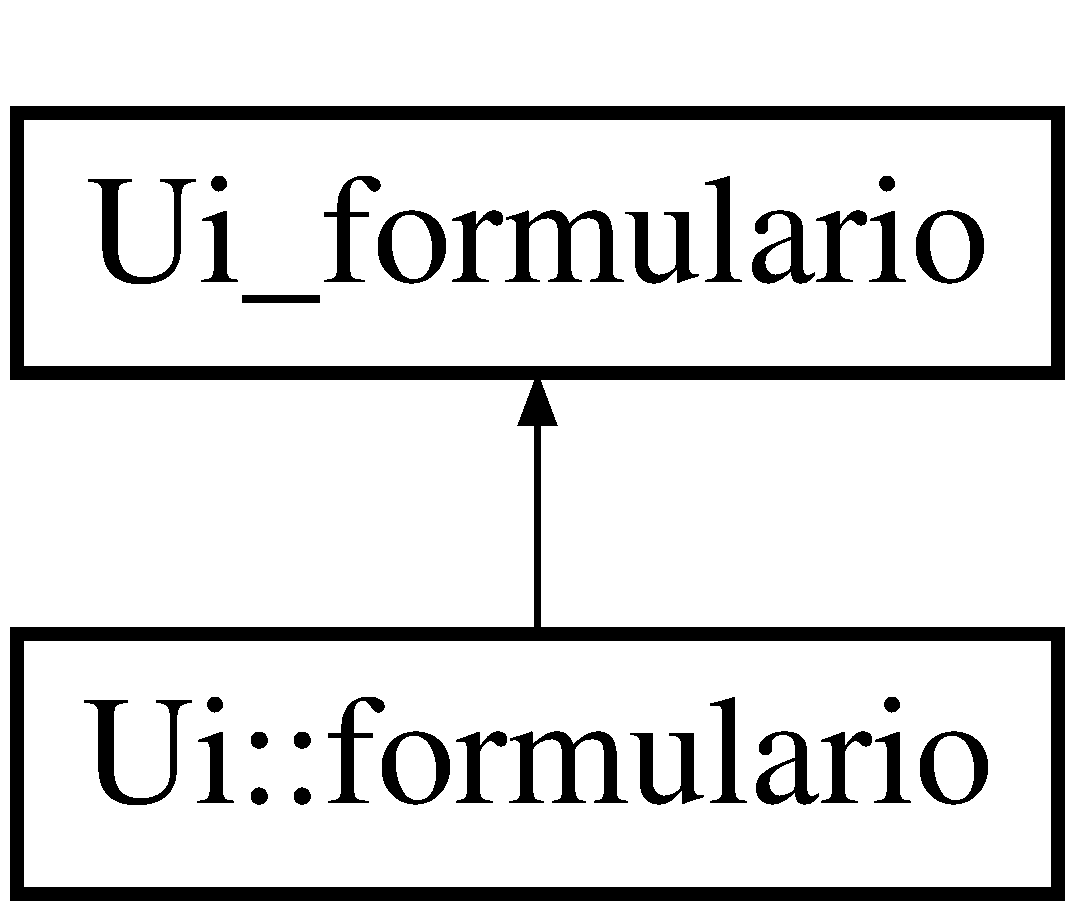
\includegraphics[height=2.000000cm]{class_ui__formulario}
\end{center}
\end{figure}
\subsection*{Public Member Functions}
\begin{DoxyCompactItemize}
\item 
\mbox{\Hypertarget{class_ui__formulario_a1e306ef2fc8720695bbcd0f9c0a4033a}\label{class_ui__formulario_a1e306ef2fc8720695bbcd0f9c0a4033a}} 
void {\bfseries setup\+Ui} (Q\+Widget $\ast$\hyperlink{classformulario}{formulario})
\item 
\mbox{\Hypertarget{class_ui__formulario_a0945c2c0fa76524453b77a93ad108467}\label{class_ui__formulario_a0945c2c0fa76524453b77a93ad108467}} 
void {\bfseries retranslate\+Ui} (Q\+Widget $\ast$\hyperlink{classformulario}{formulario})
\end{DoxyCompactItemize}
\subsection*{Public Attributes}
\begin{DoxyCompactItemize}
\item 
\mbox{\Hypertarget{class_ui__formulario_a75ba89549b5f4e6f4c0e7d2f4c19eea2}\label{class_ui__formulario_a75ba89549b5f4e6f4c0e7d2f4c19eea2}} 
Q\+Widget $\ast$ {\bfseries layout\+Widget}
\item 
\mbox{\Hypertarget{class_ui__formulario_a2a6fe4ec3d434c62abbb678569a88deb}\label{class_ui__formulario_a2a6fe4ec3d434c62abbb678569a88deb}} 
Q\+Grid\+Layout $\ast$ {\bfseries grid\+Layout\+\_\+2}
\item 
\mbox{\Hypertarget{class_ui__formulario_a72a64b74e341e65235d607690dfa6afe}\label{class_ui__formulario_a72a64b74e341e65235d607690dfa6afe}} 
Q\+H\+Box\+Layout $\ast$ {\bfseries horizontal\+Layout\+\_\+2}
\item 
\mbox{\Hypertarget{class_ui__formulario_a3a30b1eb5c25a6603bff1b13398b8fa9}\label{class_ui__formulario_a3a30b1eb5c25a6603bff1b13398b8fa9}} 
Q\+Label $\ast$ {\bfseries label\+\_\+9}
\item 
\mbox{\Hypertarget{class_ui__formulario_a30db5e6da62801b71cd8ba4cf74a34c4}\label{class_ui__formulario_a30db5e6da62801b71cd8ba4cf74a34c4}} 
Q\+Label $\ast$ {\bfseries \+\_\+nombre\+\_\+usu}
\item 
\mbox{\Hypertarget{class_ui__formulario_ac0710c15068d38e411a015b6e4436b0a}\label{class_ui__formulario_ac0710c15068d38e411a015b6e4436b0a}} 
Q\+Label $\ast$ {\bfseries label\+\_\+10}
\item 
\mbox{\Hypertarget{class_ui__formulario_a7af5440e70841968714bc22da8769192}\label{class_ui__formulario_a7af5440e70841968714bc22da8769192}} 
Q\+Label $\ast$ {\bfseries \+\_\+edad\+\_\+usuar}
\item 
\mbox{\Hypertarget{class_ui__formulario_a97d8024ea627ecc71b1e1ab4e498c34b}\label{class_ui__formulario_a97d8024ea627ecc71b1e1ab4e498c34b}} 
Q\+V\+Box\+Layout $\ast$ {\bfseries vertical\+Layout\+\_\+2}
\item 
\mbox{\Hypertarget{class_ui__formulario_a65dc56631147358bc3f8b383239c5279}\label{class_ui__formulario_a65dc56631147358bc3f8b383239c5279}} 
Q\+Grid\+Layout $\ast$ {\bfseries grid\+Layout}
\item 
\mbox{\Hypertarget{class_ui__formulario_a882195e1cc65efbecd4a09a4a2c2f325}\label{class_ui__formulario_a882195e1cc65efbecd4a09a4a2c2f325}} 
Q\+Label $\ast$ {\bfseries label\+\_\+6}
\item 
\mbox{\Hypertarget{class_ui__formulario_a9c65c2f254654a2ccc3064279b3f3503}\label{class_ui__formulario_a9c65c2f254654a2ccc3064279b3f3503}} 
Q\+Combo\+Box $\ast$ {\bfseries Genero\+\_\+r}
\item 
\mbox{\Hypertarget{class_ui__formulario_a2e1ff1c87331af96c398d316a652575e}\label{class_ui__formulario_a2e1ff1c87331af96c398d316a652575e}} 
Q\+Line\+Edit $\ast$ {\bfseries nombre\+\_\+f}
\item 
\mbox{\Hypertarget{class_ui__formulario_a4b29deb2e4a143f586811fc15730b400}\label{class_ui__formulario_a4b29deb2e4a143f586811fc15730b400}} 
Q\+Label $\ast$ {\bfseries label\+\_\+5}
\item 
\mbox{\Hypertarget{class_ui__formulario_a6f490e1e17773c497a951d3d62904e78}\label{class_ui__formulario_a6f490e1e17773c497a951d3d62904e78}} 
Q\+Line\+Edit $\ast$ {\bfseries doc\+\_\+f}
\item 
\mbox{\Hypertarget{class_ui__formulario_aaf91f1799055e46326145abdef342cb0}\label{class_ui__formulario_aaf91f1799055e46326145abdef342cb0}} 
Q\+Line\+Edit $\ast$ {\bfseries direccion\+\_\+f}
\item 
\mbox{\Hypertarget{class_ui__formulario_ac6491d58f8d49471c528839e33a77a69}\label{class_ui__formulario_ac6491d58f8d49471c528839e33a77a69}} 
Q\+Line\+Edit $\ast$ {\bfseries apellido\+\_\+f}
\item 
\mbox{\Hypertarget{class_ui__formulario_a205a19970a072dea483cd4a3d9d3f110}\label{class_ui__formulario_a205a19970a072dea483cd4a3d9d3f110}} 
Q\+Label $\ast$ {\bfseries label\+\_\+2}
\item 
\mbox{\Hypertarget{class_ui__formulario_a22a09754c19d7f43591c60225bb93470}\label{class_ui__formulario_a22a09754c19d7f43591c60225bb93470}} 
Q\+Combo\+Box $\ast$ {\bfseries Raza\+\_\+r}
\item 
\mbox{\Hypertarget{class_ui__formulario_a9f67fc4a5c968337de6225d73b93a47c}\label{class_ui__formulario_a9f67fc4a5c968337de6225d73b93a47c}} 
Q\+Label $\ast$ {\bfseries label\+\_\+4}
\item 
\mbox{\Hypertarget{class_ui__formulario_a6bad3061121b20dd6e13b1e12654c05d}\label{class_ui__formulario_a6bad3061121b20dd6e13b1e12654c05d}} 
Q\+Line\+Edit $\ast$ {\bfseries fecha\+\_\+f}
\item 
\mbox{\Hypertarget{class_ui__formulario_a43d8f7ced58143436bcc778e0b5a00ba}\label{class_ui__formulario_a43d8f7ced58143436bcc778e0b5a00ba}} 
Q\+Label $\ast$ {\bfseries label\+\_\+8}
\item 
\mbox{\Hypertarget{class_ui__formulario_a2a698aea5bc8132261a0ba27a512f492}\label{class_ui__formulario_a2a698aea5bc8132261a0ba27a512f492}} 
Q\+Label $\ast$ {\bfseries label\+\_\+7}
\item 
\mbox{\Hypertarget{class_ui__formulario_a3d5db997713bc30a9f20d16092441080}\label{class_ui__formulario_a3d5db997713bc30a9f20d16092441080}} 
Q\+Line\+Edit $\ast$ {\bfseries nivel\+\_\+f}
\item 
\mbox{\Hypertarget{class_ui__formulario_a4eef5c0c7669bbe578b530c5f025a872}\label{class_ui__formulario_a4eef5c0c7669bbe578b530c5f025a872}} 
Q\+Label $\ast$ {\bfseries label\+\_\+11}
\item 
\mbox{\Hypertarget{class_ui__formulario_a01aa3e6190f0def8916f1de5fdbc2a19}\label{class_ui__formulario_a01aa3e6190f0def8916f1de5fdbc2a19}} 
Q\+Label $\ast$ {\bfseries label}
\item 
\mbox{\Hypertarget{class_ui__formulario_a611d0d4995c49e0ae456fa4547049722}\label{class_ui__formulario_a611d0d4995c49e0ae456fa4547049722}} 
Q\+Label $\ast$ {\bfseries label\+\_\+3}
\item 
\mbox{\Hypertarget{class_ui__formulario_a06dc5970f85d46fc441d0b9cc7a07ed9}\label{class_ui__formulario_a06dc5970f85d46fc441d0b9cc7a07ed9}} 
Q\+V\+Box\+Layout $\ast$ {\bfseries vertical\+Layout}
\item 
\mbox{\Hypertarget{class_ui__formulario_a10c6c602eb53bc4080d499f28e759993}\label{class_ui__formulario_a10c6c602eb53bc4080d499f28e759993}} 
Q\+Group\+Box $\ast$ {\bfseries group\+Box}
\item 
\mbox{\Hypertarget{class_ui__formulario_ade4529bd28a172fb01439ca729a6d941}\label{class_ui__formulario_ade4529bd28a172fb01439ca729a6d941}} 
Q\+H\+Box\+Layout $\ast$ {\bfseries horizontal\+Layout\+\_\+3}
\item 
\mbox{\Hypertarget{class_ui__formulario_a663e6cc3bc1fb2dcfafe9eb21c73d77c}\label{class_ui__formulario_a663e6cc3bc1fb2dcfafe9eb21c73d77c}} 
Q\+Radio\+Button $\ast$ {\bfseries \+\_\+time30}
\item 
\mbox{\Hypertarget{class_ui__formulario_ab0008ff96eedba3e8950fd21e0ed63b6}\label{class_ui__formulario_ab0008ff96eedba3e8950fd21e0ed63b6}} 
Q\+Radio\+Button $\ast$ {\bfseries \+\_\+time1m}
\item 
\mbox{\Hypertarget{class_ui__formulario_a81f140f35ac785327f4f0750bc49a52a}\label{class_ui__formulario_a81f140f35ac785327f4f0750bc49a52a}} 
Q\+Radio\+Button $\ast$ {\bfseries \+\_\+time2m}
\item 
\mbox{\Hypertarget{class_ui__formulario_aba283363cef42f80b2b58fe963ceb497}\label{class_ui__formulario_aba283363cef42f80b2b58fe963ceb497}} 
Q\+H\+Box\+Layout $\ast$ {\bfseries horizontal\+Layout}
\item 
\mbox{\Hypertarget{class_ui__formulario_ae3320a587fcb6b360a9de7026ccb8d3b}\label{class_ui__formulario_ae3320a587fcb6b360a9de7026ccb8d3b}} 
Q\+Push\+Button $\ast$ {\bfseries iniciar\+\_\+f}
\item 
\mbox{\Hypertarget{class_ui__formulario_a5b382fc89d08aab8d3e27e67c2a845bc}\label{class_ui__formulario_a5b382fc89d08aab8d3e27e67c2a845bc}} 
Q\+Push\+Button $\ast$ {\bfseries salir\+\_\+f}
\end{DoxyCompactItemize}


The documentation for this class was generated from the following file\+:\begin{DoxyCompactItemize}
\item 
/home/alseuser/\+Descargas/\+Proyect\+\_\+\+A\+L\+S\+E\+\_\+final/\+Proyect\+\_\+\+A\+L\+S\+E/build/proyecto\+\_\+\+A\+L\+S\+E\+\_\+gui\+\_\+autogen/include/ui\+\_\+formulario.\+h\end{DoxyCompactItemize}

\hypertarget{class_ui__main__app}{}\section{Ui\+\_\+main\+\_\+app Class Reference}
\label{class_ui__main__app}\index{Ui\+\_\+main\+\_\+app@{Ui\+\_\+main\+\_\+app}}
Inheritance diagram for Ui\+\_\+main\+\_\+app\+:\begin{figure}[H]
\begin{center}
\leavevmode
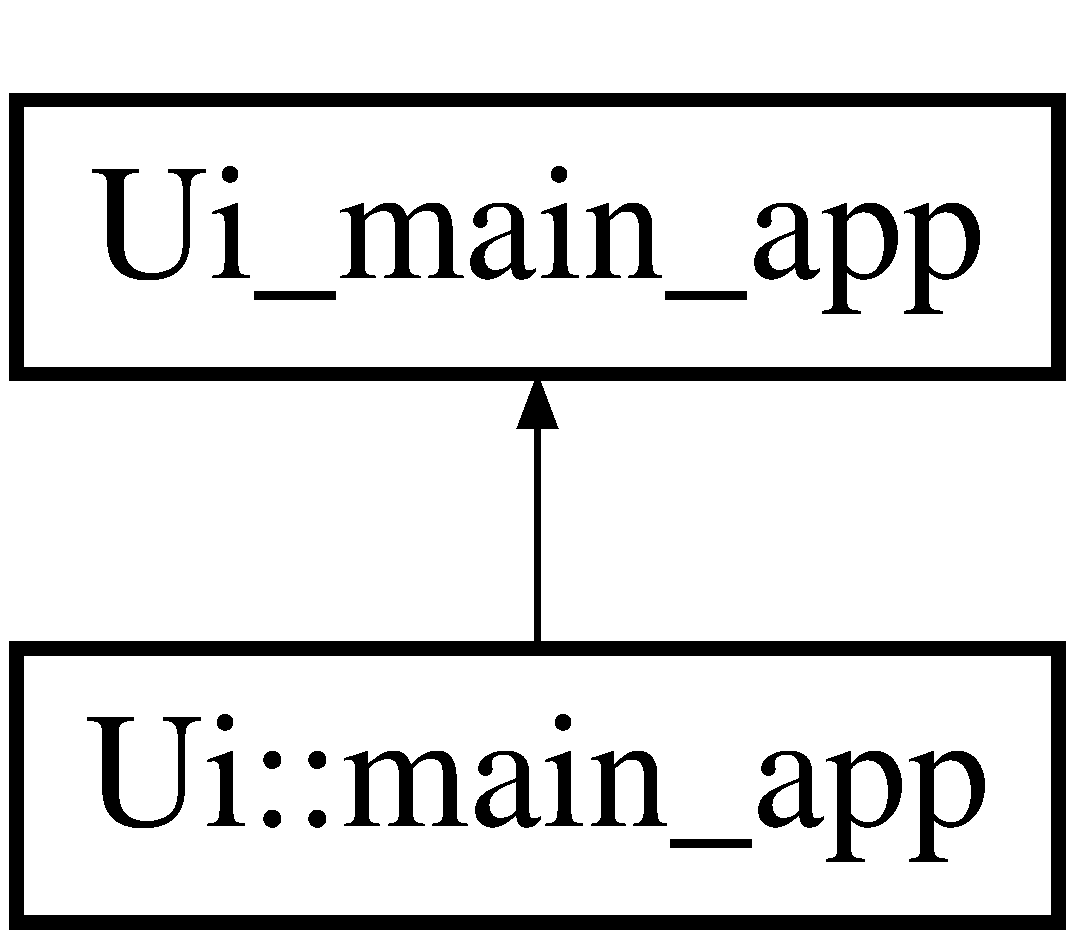
\includegraphics[height=2.000000cm]{class_ui__main__app}
\end{center}
\end{figure}
\subsection*{Public Member Functions}
\begin{DoxyCompactItemize}
\item 
\mbox{\Hypertarget{class_ui__main__app_a871b21b48d08ff6e883ea1d6e2802c2f}\label{class_ui__main__app_a871b21b48d08ff6e883ea1d6e2802c2f}} 
void {\bfseries setup\+Ui} (Q\+Main\+Window $\ast$\hyperlink{classmain__app}{main\+\_\+app})
\item 
\mbox{\Hypertarget{class_ui__main__app_a2410d167474fef942bfe02515f309a93}\label{class_ui__main__app_a2410d167474fef942bfe02515f309a93}} 
void {\bfseries retranslate\+Ui} (Q\+Main\+Window $\ast$\hyperlink{classmain__app}{main\+\_\+app})
\end{DoxyCompactItemize}
\subsection*{Public Attributes}
\begin{DoxyCompactItemize}
\item 
\mbox{\Hypertarget{class_ui__main__app_ad0202c9cb8cd2502dc7360af726e5a75}\label{class_ui__main__app_ad0202c9cb8cd2502dc7360af726e5a75}} 
Q\+Widget $\ast$ {\bfseries central\+Widget}
\item 
\mbox{\Hypertarget{class_ui__main__app_a3b4f56c1226e951beff82a9df894a702}\label{class_ui__main__app_a3b4f56c1226e951beff82a9df894a702}} 
Q\+Group\+Box $\ast$ {\bfseries group\+Box}
\item 
\mbox{\Hypertarget{class_ui__main__app_afaad9988821fe51d5c2499ba8c3d5bc8}\label{class_ui__main__app_afaad9988821fe51d5c2499ba8c3d5bc8}} 
Q\+Grid\+Layout $\ast$ {\bfseries grid\+Layout}
\item 
\mbox{\Hypertarget{class_ui__main__app_a09acc4cc448203da7788cb4b8ecf535a}\label{class_ui__main__app_a09acc4cc448203da7788cb4b8ecf535a}} 
Q\+Splitter $\ast$ {\bfseries splitter\+\_\+2}
\item 
\mbox{\Hypertarget{class_ui__main__app_a9874cbd82ffc2109838dcfc15e2c1c11}\label{class_ui__main__app_a9874cbd82ffc2109838dcfc15e2c1c11}} 
Q\+Splitter $\ast$ {\bfseries splitter}
\item 
\mbox{\Hypertarget{class_ui__main__app_ae0f65c1e84ec7e180c716d0f94ba585b}\label{class_ui__main__app_ae0f65c1e84ec7e180c716d0f94ba585b}} 
Q\+V\+Box\+Layout $\ast$ {\bfseries vertical\+Layout}
\item 
\mbox{\Hypertarget{class_ui__main__app_a4c398d3f558796098c18ed9b0a4555a4}\label{class_ui__main__app_a4c398d3f558796098c18ed9b0a4555a4}} 
Q\+H\+Box\+Layout $\ast$ {\bfseries horizontal\+Layout}
\item 
\mbox{\Hypertarget{class_ui__main__app_a4f61194d4fecb8561691eff11b7fa006}\label{class_ui__main__app_a4f61194d4fecb8561691eff11b7fa006}} 
Q\+Spacer\+Item $\ast$ {\bfseries horizontal\+Spacer}
\item 
\mbox{\Hypertarget{class_ui__main__app_adaf025a98367c473970ba45ac71bece5}\label{class_ui__main__app_adaf025a98367c473970ba45ac71bece5}} 
Q\+Push\+Button $\ast$ {\bfseries bt1}
\item 
\mbox{\Hypertarget{class_ui__main__app_a0315ac6c4177ec97e76c0f692aa9024f}\label{class_ui__main__app_a0315ac6c4177ec97e76c0f692aa9024f}} 
Q\+Spacer\+Item $\ast$ {\bfseries horizontal\+Spacer\+\_\+2}
\item 
\mbox{\Hypertarget{class_ui__main__app_a01a276827da6ed9831c28a6ab8314bc7}\label{class_ui__main__app_a01a276827da6ed9831c28a6ab8314bc7}} 
Q\+Push\+Button $\ast$ {\bfseries bt2}
\item 
\mbox{\Hypertarget{class_ui__main__app_a40a7692da4b1273f77d1043f4b2d2c0c}\label{class_ui__main__app_a40a7692da4b1273f77d1043f4b2d2c0c}} 
Q\+Spacer\+Item $\ast$ {\bfseries horizontal\+Spacer\+\_\+3}
\item 
\mbox{\Hypertarget{class_ui__main__app_abfe44c0741719d0aaa887aaf794b6391}\label{class_ui__main__app_abfe44c0741719d0aaa887aaf794b6391}} 
Q\+Push\+Button $\ast$ {\bfseries bt3}
\item 
\mbox{\Hypertarget{class_ui__main__app_aa6de655ba738a050577f8dbcb8d89436}\label{class_ui__main__app_aa6de655ba738a050577f8dbcb8d89436}} 
Q\+Spacer\+Item $\ast$ {\bfseries horizontal\+Spacer\+\_\+4}
\item 
\mbox{\Hypertarget{class_ui__main__app_aa67582f419a5cfda339ab5f278bf288e}\label{class_ui__main__app_aa67582f419a5cfda339ab5f278bf288e}} 
Q\+Push\+Button $\ast$ {\bfseries bt4}
\item 
\mbox{\Hypertarget{class_ui__main__app_a9894ff929391ac35e0a4c35bd7a9f60a}\label{class_ui__main__app_a9894ff929391ac35e0a4c35bd7a9f60a}} 
Q\+Spacer\+Item $\ast$ {\bfseries horizontal\+Spacer\+\_\+5}
\item 
\mbox{\Hypertarget{class_ui__main__app_a99a0e90e7a74adbfd67c12831e713232}\label{class_ui__main__app_a99a0e90e7a74adbfd67c12831e713232}} 
Q\+Push\+Button $\ast$ {\bfseries bt5}
\item 
\mbox{\Hypertarget{class_ui__main__app_a6e75090a6a44a9fdc0f4ebab84544233}\label{class_ui__main__app_a6e75090a6a44a9fdc0f4ebab84544233}} 
Q\+Spacer\+Item $\ast$ {\bfseries horizontal\+Spacer\+\_\+6}
\item 
\mbox{\Hypertarget{class_ui__main__app_a25238d387993b08584b0ea3e0f4bbf35}\label{class_ui__main__app_a25238d387993b08584b0ea3e0f4bbf35}} 
Q\+H\+Box\+Layout $\ast$ {\bfseries horizontal\+Layout\+\_\+2}
\item 
\mbox{\Hypertarget{class_ui__main__app_a82889ab77c09e355994f2dd1c8bc38be}\label{class_ui__main__app_a82889ab77c09e355994f2dd1c8bc38be}} 
Q\+Push\+Button $\ast$ {\bfseries bt6}
\item 
\mbox{\Hypertarget{class_ui__main__app_a3a4c8f235add1fe38bb0e40679a517ac}\label{class_ui__main__app_a3a4c8f235add1fe38bb0e40679a517ac}} 
Q\+Spacer\+Item $\ast$ {\bfseries horizontal\+Spacer\+\_\+7}
\item 
\mbox{\Hypertarget{class_ui__main__app_a6f42f5f5a0807f653d5e93d43d4620bf}\label{class_ui__main__app_a6f42f5f5a0807f653d5e93d43d4620bf}} 
Q\+Push\+Button $\ast$ {\bfseries bt7}
\item 
\mbox{\Hypertarget{class_ui__main__app_a676e9227dc1bdacfec7acc85502748a6}\label{class_ui__main__app_a676e9227dc1bdacfec7acc85502748a6}} 
Q\+Spacer\+Item $\ast$ {\bfseries horizontal\+Spacer\+\_\+9}
\item 
\mbox{\Hypertarget{class_ui__main__app_a4fb3f0a3cc341cb686a8ab2d5fd1e724}\label{class_ui__main__app_a4fb3f0a3cc341cb686a8ab2d5fd1e724}} 
Q\+Push\+Button $\ast$ {\bfseries bt8}
\item 
\mbox{\Hypertarget{class_ui__main__app_a59554266a396dc13c76ccc0504f01170}\label{class_ui__main__app_a59554266a396dc13c76ccc0504f01170}} 
Q\+Spacer\+Item $\ast$ {\bfseries horizontal\+Spacer\+\_\+10}
\item 
\mbox{\Hypertarget{class_ui__main__app_a480446a9c3878574cdd4c0d6ace45da1}\label{class_ui__main__app_a480446a9c3878574cdd4c0d6ace45da1}} 
Q\+Push\+Button $\ast$ {\bfseries bt9}
\item 
\mbox{\Hypertarget{class_ui__main__app_ab5b061010cb2ef2a2b19342e26843473}\label{class_ui__main__app_ab5b061010cb2ef2a2b19342e26843473}} 
Q\+Spacer\+Item $\ast$ {\bfseries horizontal\+Spacer\+\_\+8}
\item 
\mbox{\Hypertarget{class_ui__main__app_ac385a45dc76dcb3b4e9c7d7c225723ef}\label{class_ui__main__app_ac385a45dc76dcb3b4e9c7d7c225723ef}} 
Q\+Push\+Button $\ast$ {\bfseries bt10}
\item 
\mbox{\Hypertarget{class_ui__main__app_afaeb439578667bf5a1103f5a02215837}\label{class_ui__main__app_afaeb439578667bf5a1103f5a02215837}} 
Q\+Spacer\+Item $\ast$ {\bfseries horizontal\+Spacer\+\_\+11}
\item 
\mbox{\Hypertarget{class_ui__main__app_a7aadf63dc799f006e318943cf54a0ac0}\label{class_ui__main__app_a7aadf63dc799f006e318943cf54a0ac0}} 
Q\+Push\+Button $\ast$ {\bfseries bt11}
\item 
\mbox{\Hypertarget{class_ui__main__app_ad1c28e30d81ff19b625290f7a9798a94}\label{class_ui__main__app_ad1c28e30d81ff19b625290f7a9798a94}} 
Q\+Line\+Edit $\ast$ {\bfseries aciertos\+\_\+e}
\item 
\mbox{\Hypertarget{class_ui__main__app_aeb94625a8c1c4376ae509aec3a50ab41}\label{class_ui__main__app_aeb94625a8c1c4376ae509aec3a50ab41}} 
Q\+Label $\ast$ {\bfseries label}
\item 
\mbox{\Hypertarget{class_ui__main__app_afd886e7ada9f507e47537dd1cf6d6b4f}\label{class_ui__main__app_afd886e7ada9f507e47537dd1cf6d6b4f}} 
Q\+Label $\ast$ {\bfseries label\+\_\+2}
\item 
\mbox{\Hypertarget{class_ui__main__app_ae5e774947efb468db8c66b36d0bc22c8}\label{class_ui__main__app_ae5e774947efb468db8c66b36d0bc22c8}} 
Q\+Line\+Edit $\ast$ {\bfseries line\+Edit}
\item 
\mbox{\Hypertarget{class_ui__main__app_a7f8aa699e38eab18549932caab4992c7}\label{class_ui__main__app_a7f8aa699e38eab18549932caab4992c7}} 
Q\+Menu\+Bar $\ast$ {\bfseries menu\+Bar}
\item 
\mbox{\Hypertarget{class_ui__main__app_a9e56f426088a781f6a01dc11e110668f}\label{class_ui__main__app_a9e56f426088a781f6a01dc11e110668f}} 
Q\+Tool\+Bar $\ast$ {\bfseries main\+Tool\+Bar}
\item 
\mbox{\Hypertarget{class_ui__main__app_a00d5194852ac5f91f61b26f9d99f688e}\label{class_ui__main__app_a00d5194852ac5f91f61b26f9d99f688e}} 
Q\+Status\+Bar $\ast$ {\bfseries status\+Bar}
\end{DoxyCompactItemize}


The documentation for this class was generated from the following file\+:\begin{DoxyCompactItemize}
\item 
/home/alseuser/\+Descargas/\+Proyect\+\_\+\+A\+L\+S\+E\+\_\+final/\+Proyect\+\_\+\+A\+L\+S\+E/build/proyecto\+\_\+\+A\+L\+S\+E\+\_\+gui\+\_\+autogen/include/ui\+\_\+main\+\_\+app.\+h\end{DoxyCompactItemize}

\hypertarget{class_ui__plataforma}{}\section{Ui\+\_\+plataforma Class Reference}
\label{class_ui__plataforma}\index{Ui\+\_\+plataforma@{Ui\+\_\+plataforma}}
Inheritance diagram for Ui\+\_\+plataforma\+:\begin{figure}[H]
\begin{center}
\leavevmode
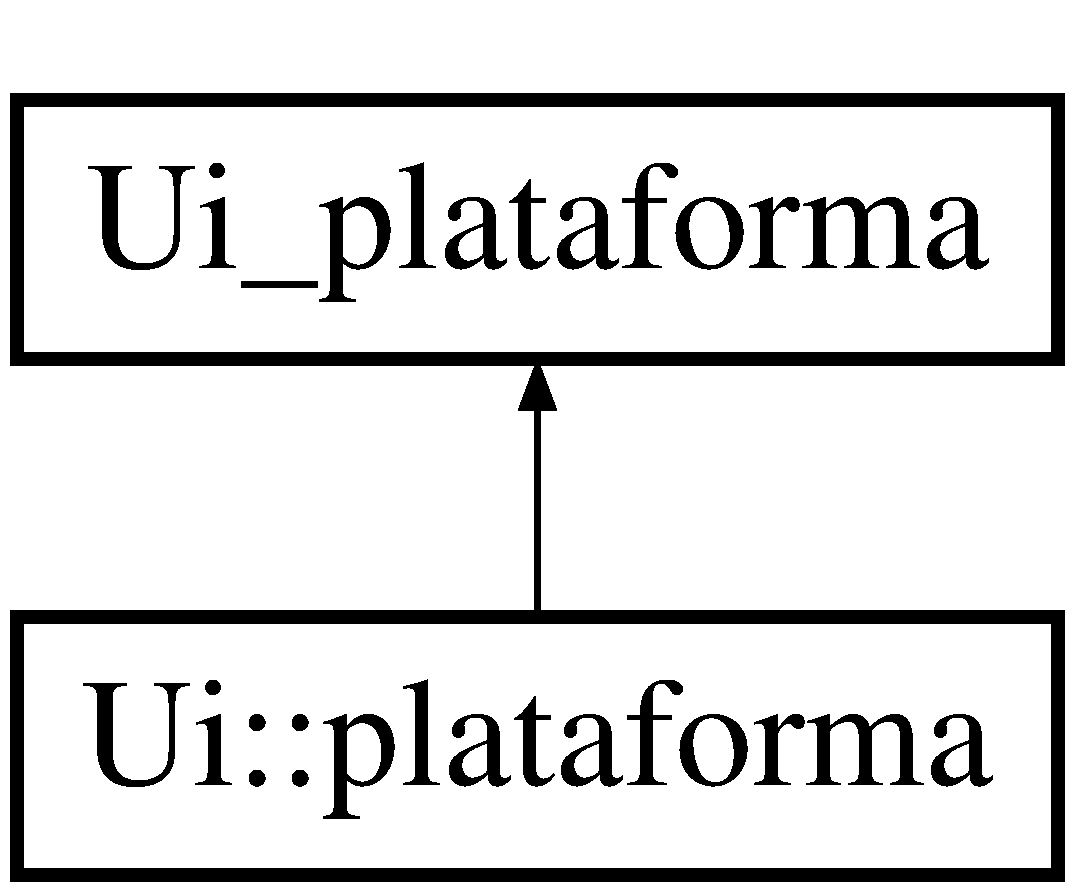
\includegraphics[height=2.000000cm]{class_ui__plataforma}
\end{center}
\end{figure}
\subsection*{Public Member Functions}
\begin{DoxyCompactItemize}
\item 
\mbox{\Hypertarget{class_ui__plataforma_a5ac882befb022b15a571bcd5589dbacb}\label{class_ui__plataforma_a5ac882befb022b15a571bcd5589dbacb}} 
void {\bfseries setup\+Ui} (Q\+Widget $\ast$\hyperlink{classplataforma}{plataforma})
\item 
\mbox{\Hypertarget{class_ui__plataforma_aae918034c87c91b40e1ecccab8b5cbd0}\label{class_ui__plataforma_aae918034c87c91b40e1ecccab8b5cbd0}} 
void {\bfseries retranslate\+Ui} (Q\+Widget $\ast$\hyperlink{classplataforma}{plataforma})
\end{DoxyCompactItemize}
\subsection*{Public Attributes}
\begin{DoxyCompactItemize}
\item 
\mbox{\Hypertarget{class_ui__plataforma_a51da2e185c7ea1710fbde908f5106170}\label{class_ui__plataforma_a51da2e185c7ea1710fbde908f5106170}} 
Q\+Label $\ast$ {\bfseries label}
\item 
\mbox{\Hypertarget{class_ui__plataforma_ab4df0b904987b2904c9f798389773758}\label{class_ui__plataforma_ab4df0b904987b2904c9f798389773758}} 
Q\+Push\+Button $\ast$ {\bfseries registro\+\_\+p}
\item 
\mbox{\Hypertarget{class_ui__plataforma_aa33f7d9fce2a49ae56ac0d543c27e6ca}\label{class_ui__plataforma_aa33f7d9fce2a49ae56ac0d543c27e6ca}} 
Q\+Line\+Edit $\ast$ {\bfseries password\+\_\+p}
\item 
\mbox{\Hypertarget{class_ui__plataforma_a07d674ab7e63711328b006cbe0b86a8d}\label{class_ui__plataforma_a07d674ab7e63711328b006cbe0b86a8d}} 
Q\+Label $\ast$ {\bfseries label\+\_\+3}
\item 
\mbox{\Hypertarget{class_ui__plataforma_aa14326d047614f6752e37fe81997024c}\label{class_ui__plataforma_aa14326d047614f6752e37fe81997024c}} 
Q\+Line\+Edit $\ast$ {\bfseries Restriccion\+\_\+p}
\item 
\mbox{\Hypertarget{class_ui__plataforma_ae7fc2481ca0506b42228c381e01fd8a4}\label{class_ui__plataforma_ae7fc2481ca0506b42228c381e01fd8a4}} 
Q\+Line\+Edit $\ast$ {\bfseries nombre\+\_\+p}
\item 
\mbox{\Hypertarget{class_ui__plataforma_a8b852efa478ee8e28a7d92e9c1955b5e}\label{class_ui__plataforma_a8b852efa478ee8e28a7d92e9c1955b5e}} 
Q\+Push\+Button $\ast$ {\bfseries ingreso\+\_\+p}
\item 
\mbox{\Hypertarget{class_ui__plataforma_ae4475a26e88351577bf11dabf3e4e45e}\label{class_ui__plataforma_ae4475a26e88351577bf11dabf3e4e45e}} 
Q\+Label $\ast$ {\bfseries label\+\_\+2}
\end{DoxyCompactItemize}


The documentation for this class was generated from the following file\+:\begin{DoxyCompactItemize}
\item 
/home/alseuser/\+Descargas/\+Proyect\+\_\+\+A\+L\+S\+E\+\_\+final/\+Proyect\+\_\+\+A\+L\+S\+E/build/proyecto\+\_\+\+A\+L\+S\+E\+\_\+gui\+\_\+autogen/include/ui\+\_\+plataforma.\+h\end{DoxyCompactItemize}

\hypertarget{class_ui__registro}{}\section{Ui\+\_\+registro Class Reference}
\label{class_ui__registro}\index{Ui\+\_\+registro@{Ui\+\_\+registro}}
Inheritance diagram for Ui\+\_\+registro\+:\begin{figure}[H]
\begin{center}
\leavevmode
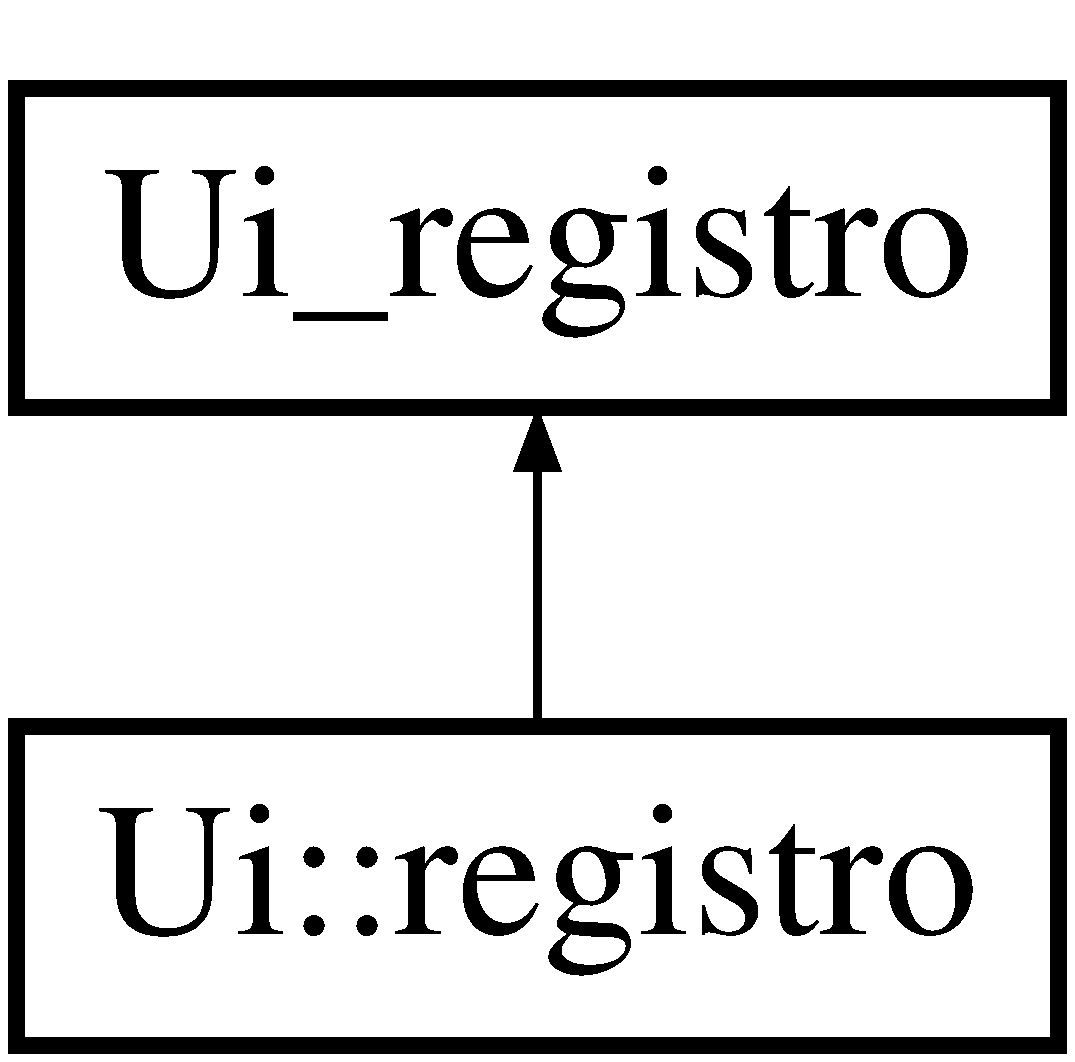
\includegraphics[height=2.000000cm]{class_ui__registro}
\end{center}
\end{figure}
\subsection*{Public Member Functions}
\begin{DoxyCompactItemize}
\item 
\mbox{\Hypertarget{class_ui__registro_a35262f801bcc8d2d7cd712cb88dcc265}\label{class_ui__registro_a35262f801bcc8d2d7cd712cb88dcc265}} 
void {\bfseries setup\+Ui} (Q\+Widget $\ast$\hyperlink{classregistro}{registro})
\item 
\mbox{\Hypertarget{class_ui__registro_a862cab2b7154b318c2ec1ef283bfd0dd}\label{class_ui__registro_a862cab2b7154b318c2ec1ef283bfd0dd}} 
void {\bfseries retranslate\+Ui} (Q\+Widget $\ast$\hyperlink{classregistro}{registro})
\end{DoxyCompactItemize}
\subsection*{Public Attributes}
\begin{DoxyCompactItemize}
\item 
\mbox{\Hypertarget{class_ui__registro_afd1328f721d8acfb6c9323757174aea2}\label{class_ui__registro_afd1328f721d8acfb6c9323757174aea2}} 
Q\+Widget $\ast$ {\bfseries layout\+Widget}
\item 
\mbox{\Hypertarget{class_ui__registro_ae9027a1de2aae9c7965c2be9830f161e}\label{class_ui__registro_ae9027a1de2aae9c7965c2be9830f161e}} 
Q\+Grid\+Layout $\ast$ {\bfseries grid\+Layout}
\item 
\mbox{\Hypertarget{class_ui__registro_a2306c9d4eaaba2ba9a18fe04e6a8778d}\label{class_ui__registro_a2306c9d4eaaba2ba9a18fe04e6a8778d}} 
Q\+Line\+Edit $\ast$ {\bfseries nombre\+\_\+r}
\item 
\mbox{\Hypertarget{class_ui__registro_a5e8f8cc159d708a1ee2e66145e822f87}\label{class_ui__registro_a5e8f8cc159d708a1ee2e66145e822f87}} 
Q\+Label $\ast$ {\bfseries label\+\_\+4}
\item 
\mbox{\Hypertarget{class_ui__registro_a8d0398abebac5e47cfff7b89f973bef4}\label{class_ui__registro_a8d0398abebac5e47cfff7b89f973bef4}} 
Q\+Push\+Button $\ast$ {\bfseries registro\+\_\+r}
\item 
\mbox{\Hypertarget{class_ui__registro_a9d4057b53d36eb1f83aec92959d79d85}\label{class_ui__registro_a9d4057b53d36eb1f83aec92959d79d85}} 
Q\+Label $\ast$ {\bfseries label}
\item 
\mbox{\Hypertarget{class_ui__registro_a836a6342288da3272197b13b182769f0}\label{class_ui__registro_a836a6342288da3272197b13b182769f0}} 
Q\+Label $\ast$ {\bfseries label\+\_\+7}
\item 
\mbox{\Hypertarget{class_ui__registro_a310b11b1fd9d2efad1e19fe1ec9f4064}\label{class_ui__registro_a310b11b1fd9d2efad1e19fe1ec9f4064}} 
Q\+Label $\ast$ {\bfseries label\+\_\+2}
\item 
\mbox{\Hypertarget{class_ui__registro_a487e53fbc36b86710ccb8bf1366c5944}\label{class_ui__registro_a487e53fbc36b86710ccb8bf1366c5944}} 
Q\+Label $\ast$ {\bfseries label\+\_\+3}
\item 
\mbox{\Hypertarget{class_ui__registro_ab16f41253575c0b8ed6f9cb542132d97}\label{class_ui__registro_ab16f41253575c0b8ed6f9cb542132d97}} 
Q\+Line\+Edit $\ast$ {\bfseries doc\+\_\+r}
\item 
\mbox{\Hypertarget{class_ui__registro_ae1d5af9251fd65445aa60eb5003847fa}\label{class_ui__registro_ae1d5af9251fd65445aa60eb5003847fa}} 
Q\+Push\+Button $\ast$ {\bfseries cancelar\+\_\+r}
\item 
\mbox{\Hypertarget{class_ui__registro_ab52a49005a5c2321bf0548e857fce550}\label{class_ui__registro_ab52a49005a5c2321bf0548e857fce550}} 
Q\+Line\+Edit $\ast$ {\bfseries fecha\+\_\+r}
\item 
\mbox{\Hypertarget{class_ui__registro_a424368ae2a7ca67cbd0139b63db50435}\label{class_ui__registro_a424368ae2a7ca67cbd0139b63db50435}} 
Q\+Line\+Edit $\ast$ {\bfseries apellido\+\_\+r}
\item 
\mbox{\Hypertarget{class_ui__registro_aae27d1f2c608740c0153a9e0477e9944}\label{class_ui__registro_aae27d1f2c608740c0153a9e0477e9944}} 
Q\+Label $\ast$ {\bfseries label\+\_\+8}
\item 
\mbox{\Hypertarget{class_ui__registro_a2e63263b02c60fc2a089893c651daf53}\label{class_ui__registro_a2e63263b02c60fc2a089893c651daf53}} 
Q\+Line\+Edit $\ast$ {\bfseries Com\+\_\+fecha}
\item 
\mbox{\Hypertarget{class_ui__registro_ab6d06916f3d816934ad5b656ed33af37}\label{class_ui__registro_ab6d06916f3d816934ad5b656ed33af37}} 
Q\+Line\+Edit $\ast$ {\bfseries pasword\+\_\+r}
\item 
\mbox{\Hypertarget{class_ui__registro_a2f231c4f6b1a0012c5b77c2265983d81}\label{class_ui__registro_a2f231c4f6b1a0012c5b77c2265983d81}} 
Q\+Line\+Edit $\ast$ {\bfseries User\+\_\+r}
\item 
\mbox{\Hypertarget{class_ui__registro_a936008048ab955b86177c680bb580bdc}\label{class_ui__registro_a936008048ab955b86177c680bb580bdc}} 
Q\+Label $\ast$ {\bfseries label\+\_\+6}
\item 
\mbox{\Hypertarget{class_ui__registro_a851df2843214b8e05fdd63989dc279a1}\label{class_ui__registro_a851df2843214b8e05fdd63989dc279a1}} 
Q\+Label $\ast$ {\bfseries label\+\_\+5}
\end{DoxyCompactItemize}


The documentation for this class was generated from the following file\+:\begin{DoxyCompactItemize}
\item 
/home/alseuser/\+Descargas/\+Proyect\+\_\+\+A\+L\+S\+E\+\_\+final/\+Proyect\+\_\+\+A\+L\+S\+E/build/proyecto\+\_\+\+A\+L\+S\+E\+\_\+gui\+\_\+autogen/include/ui\+\_\+registro.\+h\end{DoxyCompactItemize}

\hypertarget{classusuario}{}\section{usuario Class Reference}
\label{classusuario}\index{usuario@{usuario}}


En esta clase definimos todos los datos que se deben tener de un usuario que utilice la plataforma de registros. Las funciones fueron implementadas como funciones inline que optimizan los recursos de la maquina agilizando algunos procesos.  




{\ttfamily \#include $<$usuario.\+h$>$}

\subsection*{Public Member Functions}
\begin{DoxyCompactItemize}
\item 
\hyperlink{classusuario_a31d080a47bebcedffe122527e3389648}{usuario} ()
\item 
\mbox{\Hypertarget{classusuario_afae576238cc91e38757c09f5b223913c}\label{classusuario_afae576238cc91e38757c09f5b223913c}} 
void {\bfseries set\+Fecha} (string fecha)
\item 
\mbox{\Hypertarget{classusuario_a2b1e59077c6f3db48ec180f5a8d10d84}\label{classusuario_a2b1e59077c6f3db48ec180f5a8d10d84}} 
string {\bfseries get\+Fecha} () const
\item 
\mbox{\Hypertarget{classusuario_a03e0eb35fb6274e77e016132b907ddcc}\label{classusuario_a03e0eb35fb6274e77e016132b907ddcc}} 
void {\bfseries set\+Doc} (double Doc)
\item 
\mbox{\Hypertarget{classusuario_a59b68b87c3000a9c25aed5e82578d5e8}\label{classusuario_a59b68b87c3000a9c25aed5e82578d5e8}} 
double {\bfseries get\+Doc} () const
\item 
\mbox{\Hypertarget{classusuario_ad6a75d542d7bcf4b7c073dcb5de2e5a4}\label{classusuario_ad6a75d542d7bcf4b7c073dcb5de2e5a4}} 
void {\bfseries set\+Nombre} (string nombre)
\item 
\mbox{\Hypertarget{classusuario_a2071eb11fa831ef2a05915c8168f6a94}\label{classusuario_a2071eb11fa831ef2a05915c8168f6a94}} 
string {\bfseries get\+Nombre} () const
\item 
\mbox{\Hypertarget{classusuario_af271213c4f37acb50eb01c6741671786}\label{classusuario_af271213c4f37acb50eb01c6741671786}} 
void {\bfseries set\+Apellido} (string apellido)
\item 
\mbox{\Hypertarget{classusuario_a5189ddcbb2faff1cd493f815183b9475}\label{classusuario_a5189ddcbb2faff1cd493f815183b9475}} 
string {\bfseries get\+Apellido} () const
\item 
\mbox{\Hypertarget{classusuario_aaf2f2b6af8aa2201c6afcf4d6cfccd22}\label{classusuario_aaf2f2b6af8aa2201c6afcf4d6cfccd22}} 
void {\bfseries set\+Contrasena} (string contrasena)
\item 
\mbox{\Hypertarget{classusuario_a3e9a305e92d2c1b0f351d9b516bc3c76}\label{classusuario_a3e9a305e92d2c1b0f351d9b516bc3c76}} 
string {\bfseries get\+Contrasena} () const
\item 
\mbox{\Hypertarget{classusuario_a6afeca232fe67fa3f434e86d7e7048f6}\label{classusuario_a6afeca232fe67fa3f434e86d7e7048f6}} 
void {\bfseries set\+\_\+\+Usuario} (string user\+\_\+1)
\item 
\mbox{\Hypertarget{classusuario_ae7f5ee4ff05f174e7439b3541678b9ae}\label{classusuario_ae7f5ee4ff05f174e7439b3541678b9ae}} 
string {\bfseries get\+\_\+\+Usuario} () const
\item 
\mbox{\Hypertarget{classusuario_aa040e5b3258ad6a1878e9429603d722c}\label{classusuario_aa040e5b3258ad6a1878e9429603d722c}} 
void {\bfseries set\+\_\+edad} (int edad)
\item 
\mbox{\Hypertarget{classusuario_ada8475d0d4bc0240b5b3be3be9cb5564}\label{classusuario_ada8475d0d4bc0240b5b3be3be9cb5564}} 
int {\bfseries get\+\_\+edad} () const
\end{DoxyCompactItemize}


\subsection{Detailed Description}
En esta clase definimos todos los datos que se deben tener de un usuario que utilice la plataforma de registros. Las funciones fueron implementadas como funciones inline que optimizan los recursos de la maquina agilizando algunos procesos. 

\subsection{Constructor \& Destructor Documentation}
\mbox{\Hypertarget{classusuario_a31d080a47bebcedffe122527e3389648}\label{classusuario_a31d080a47bebcedffe122527e3389648}} 
\index{usuario@{usuario}!usuario@{usuario}}
\index{usuario@{usuario}!usuario@{usuario}}
\subsubsection{\texorpdfstring{usuario()}{usuario()}}
{\footnotesize\ttfamily usuario\+::usuario (\begin{DoxyParamCaption}{ }\end{DoxyParamCaption})}

La implementación de esta clase no es necesaria, pues se realizó por medio de funciones inline. 

The documentation for this class was generated from the following files\+:\begin{DoxyCompactItemize}
\item 
/home/alseuser/\+Descargas/\+Proyect\+\_\+\+A\+L\+S\+E\+\_\+final/\+Proyect\+\_\+\+A\+L\+S\+E/usuario.\+h\item 
/home/alseuser/\+Descargas/\+Proyect\+\_\+\+A\+L\+S\+E\+\_\+final/\+Proyect\+\_\+\+A\+L\+S\+E/usuario.\+cpp\end{DoxyCompactItemize}

%--- End generated contents ---

% Index
\backmatter
\newpage
\phantomsection
\clearemptydoublepage
\addcontentsline{toc}{chapter}{Index}
\printindex

\end{document}
